\chapter{Analysis}
\label{chap:analysis}

This chapter is based mainly on our publication \cite{polattro} which is partially presented at 
\cite{polatACC11,polatIFAC11,polatWH11}. We introduce the IQC analysis framework to unify frequency 
based analysis results while preserving the exactness of the conditions or if any without introducing extra 
conservatism . Via numerical case studies, we show that the results are precisely the same with those of the 
techniques available in the literature. Therefore, we prove that there is no fundamental reason to use a 
specialized terminology and set of techniques out of the mainstream robust control theory.


\section{Quadratic Forms for Stability Analysis}
In the sequel, instead of 2-port networks, we rather consider system interconnections as 
depicted in \Cref{fig:uncic}. In this setting, $G$ is the model of the nominal bilateral 
teleoperation system and $\Delta$ is a block diagonal collection of uncertainties, such as 
the human, the environment, delays, etc. Stability tests are based on structural hypotheses 
on the diagonal blocks of the operator $\Delta$ such as gain bounds or passivity. These 
properties should allow us to develop numerically verifiable conditions for the system $G$ that 
guarantee interconnection stability. This is intuitive because we have no access to the actual 
$\Delta$ and we can only describe its components by means of indirect properties. Over the 
past three decades many classical stability results have been unified and generalized in 
this direction by utilizing quadratic forms (see \cite{megretski} and \cite{safonov,carsten2,iwasaki}).


\begin{figure}
\begin{subfigure}[b]{.5\linewidth}
\centering%
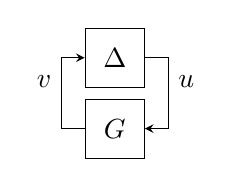
\begin{tikzpicture}[>=stealth,scale=0.6]
\node[draw,minimum size=0.75cm] (plant) at (0,0) {$G$};
\node[draw,minimum size=0.75cm] (unc) at (0,1.5) {$\Delta$};
\draw[->] (plant.west) -| ++(-5mm,10mm) node[left] {$v$} |- (unc.west);
\draw[->] (unc.east)   -| ++(5mm,-5mm) node[right] {$u$} |- (plant.east);
\end{tikzpicture}	
\caption{}\label{fig:uncic}
\end{subfigure}%
\begin{subfigure}[b]{.5\linewidth}
\centering%
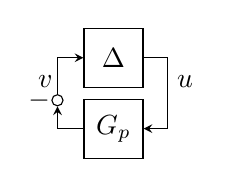
\begin{tikzpicture}[>=stealth,scale=0.6]
\node[draw,rectangle, minimum size=0.75cm] (plant) at (0,0) {$G_p$};
\node[draw,rectangle, minimum size=0.75cm] (unc) at (0,1.5cm) {$\Delta$};
\node[draw,circle,inner sep=0.5mm,label={[inner sep=0.1mm]180:$-$},label={[inner sep=0,yshift=1mm]135:$v$}] at ([shift={(-0.55cm,0.6cm)}]plant.west)(junc) {};
\draw[->] (plant.west) -| (junc.south);
\draw[->] (junc.north) |- (unc.west);
\draw[->] (unc.east) -| ++(0.5cm,-0.5cm) node[right]{$u$}|- (plant.east);
\end{tikzpicture}
\caption{}\label{fig:uncicpas}
\end{subfigure}
\caption[The general system interconnections]{The general interconnection (a) and the assumed interconnection for passive systems 
(b). In general, the power variables require a sign change relative to the ``from'' and ``to'' ports 
in order to indicate the travel direction which translates to a negative sign in the block diagrams.}
\label{fig:2}
\end{figure}

For the sake of completeness, we present the general methodology by sampling a few important special cases. 
To begin with, consider the following reformulation of the conditions of the small-gain theorem:
\begin{equation}
\begin{aligned}
\|\Delta\|_\infty &\leq 1\\
\|G\|_\infty &< 1
\end{aligned} \iff
{\scriptstyle \begin{aligned}
\pmatr{\Delta(\iw)\\1}^*\pmatr{-1 &0\\0 &1}\pmatr{\Delta(\iw)\\1} &\geq 0\\
\pmatr{1\\G(\iw)}^*\pmatr{-1 &0\\0 &1}\pmatr{1\\G(\iw)} &< 0
\end{aligned}}
\label{eq:smqf}
\end{equation}
for all $\omega\in\Realext$. The middle {$2\times2$ matrix} on the right-hand side is called the 
``\emph{multiplier}'' (typically denoted by $\Pi$). It has been observed that the appearance of the 
same multiplier on both inequalities is far from a mere coincidence. In fact, it led to the following 
stability test: Assume that $G,\Delta\in \mathcal{RH}^{\bullet \times \bullet}_\infty$. Then, the 
$G-\Delta$ interconnection {in \Cref{fig:uncic}} is well posed and stable if there exists a 
Hermitian matrix $\Pi$ such that
\begin{equation}
\pmatr{\Delta(\iw)\\I}^*\!\!\!\Pi\pmatr{\Delta(\iw)\\I} \succeq 0,\
\pmatr{I\\G(\iw)}^*\!\!\!\Pi\pmatr{I\\G(\iw)} \prec 0  \label{eq:qcdelta}
\end{equation}
hold for all $\omega\in\Realext$; one only requires the mild technical hypothesis that the left-upper/right-lower 
block of $\Pi$ is negative/positive semi-definite. Thus, the intuition that we touched upon above is mathematically 
formalized by \eqref{eq:qcdelta}. Indeed, one can see that the former condition constrains the family of uncertainties,
 while the latter {provides the related condition} imposed on the plant for interconnection stability, both expressed 
in terms of the multiplier $\Pi$. In particular, we recover the passivity theorem in a similar fashion, if {using} 
the constant symmetric matrix $\Pi=\left(\begin{smallmatrix}0 &I \\ I &0 \end{smallmatrix} \right)$ as the multiplier 
under negative feedback. See \cite{safonov} for a lucid ``topological seperation" argument. Various other classical 
stability tests fall under this particular {scenario based on the so-called static (frequency-independent) multipliers 
which, therefore, presents} a significantly unified methodology.

If $\Delta$ admits a diagonal structure (as in \Cref{fig:portrep}), it is well known that the small-gain theorem 
and passivity theorem are conservative. A natural generalization toward a tighter analysis test is using a frequency-dependent 
$\Pi$ matrix, {which can be interpreted as} adding dynamics to the multiplier. Two prominent examples of 
interest are the celebrated upper bound computations for $\mu$ or $\kappa_m$ in robust control theory and, as we will 
show later, Llewellyn's stability conditions. As a shortcoming, these results are only valid for LTI operators but the 
real power and flexibility of these multiplier methods come from {their} generalizations to classes of nonlinear/time-varying 
operators via the IQC framework that appeared in \cite{megretski}.

An IQC for the input and output signals of $\Delta$ is expressed as
\begin{equation}{\infint{\pmatr{\widehat{\Delta(v)}(\iw)\\\hat{v}(\iw)}^*\Pi(\iw)\pmatr{\widehat{\Delta(v)}(\iw)\\\hat{v}(\iw)}d\omega}} \succeq 0.
\label{eq:IQC}
\end{equation}
A bounded operator $\Delta:\mathcal{L}^m_2\to\mathcal{L}^n_2$ is said to satisfy the constraint defined by $\Pi(\iw)$ 
if \eqref{eq:IQC} holds for all $v\in\mathcal{L}^m_2$. The following sufficient {stability condition for the interconnection 
in \Cref{fig:uncic}} forms the basis for the IQC framework. 


\begin{thm}[\cite{megretski}]\label{IQCthm} Let $G\in\mathcal{RH}^{m\times n}_\infty$ be given and 
let $\Delta:\mathcal{L}^m_2\to\mathcal{L}^n_2$ be a bounded causal operator. Suppose that
\begin{enumerate}
	\item for every $\tau\in[0,1]$, the interconnection of $G$ and $\tau\Delta$ is well posed;
	\item for every $\tau\in[0,1]$, $\tau\Delta$ satisfies the IQC 
    defined by $\Pi(\iw)$ which is bounded as a function of $\omega\in\Real$;
	\item there exists some $\epsilon>0$ such that
	\begin{equation}
	\pmatr{I\\G(\iw)}^*\Pi(\iw)\pmatr{I\\G(\iw)} \preceq -\epsilon I\text{\ for all\ }\omega\in\mathbb{\Real}.
	\label{eq:IQCthmFDI}
	\end{equation}
\end{enumerate}
Then the $G-\Delta$ interconnection {in \Cref{fig:uncic}}  is stable.
\end{thm}

We include a few remarks about this result: 
\begin{rem}\label{remiqc1}
Note that both properties 1 and 2 in \Cref{IQCthm} have to hold for $\tau\Delta$ 
if $\tau$ moves from $\tau=0$ (for which stability is obvious) to the target value $\tau=1$ 
(for which stability is desired). But, the reason for using a scalar $\tau$ is to scale the uncertainty
size, therefore it does not have to be a multiplication operation, e.g., in the delay uncertainty cases,
scaling the uncertainty $\tau e^{-sT}$ is incorrect for the application of IQC theorem. Instead, 
the result can still be used if one considers $e^{-s\tau T}$ for $\tau\in[0,1]$, as we will derive
a multiplier class later in this chapter. In summary, the homotopy 
argument can be customized and  by no means limited to $\tau\Delta$. 

Let the multiplier $\Pi(\iw)$ partitioned as
\begin{equation}
\Pi = \pmatr{\Pi_1&\Pi_2\\\Pi_2^* &\Pi_3}
\label{eq:Pipart}
\end{equation}
In our examples the left-upper $m\times m$ block is negative semi-definite for all $\omega\in\Realext$
which guarantees concavity. In other words, convex combinations of two particular uncertainty element 
$\Delta_1, \Delta_2$ that satisfies the IQC, also satisfy the IQC since
\[
\pmatr{\tau\Delta_1+(1-\tau)\Delta_2\\ I}^*\pmatr{-&\cdot\\\cdot &\cdot}\pmatr{\tau\Delta_1+(1-\tau)\Delta_2\\I}
\]
is a concave function. Furthermore, we assume that the right-lower $m\times m$ block of $\Pi(\iw)$ 
positive semidefinite for all $\omega\in\Realext$. Then
\[
\pmatr{0\\I}^*\pmatr{\cdot &\cdot\\\cdot &+}\pmatr{0\\ I} \succeq 0
\]
i.e. $0\in\bm{\Delta}$.
Hence, given a $\Delta$ that satisfies the IQC with $\Pi_1 \succeq 0, \Pi_3\preceq 0$, select $\Delta_1 = 0, \Delta_2 = \Delta$, 
for every $\tau\in [0,1]$, $\tau\Delta$ satisfies the IQC. 
The reason why we are so interested in zero is the fact that when $\Delta=0$, it corresponds to the (unperturbed) nominal 
system and, as is for the IQC theorem, many stability results rely on tracking the stability property while traveling on 
the nominal system$\to$fully uncertain system path, e.g., root loci, Nyquist test, boundary crossing theorem, $\mu$-analysis
etc. 


It is then easy to see that \eqref{eq:qcdelta} implies property 2 in \Cref{IQCthm}; 
hence one only needs to verify \eqref{eq:qcdelta} for the original uncertainty $\Delta$.
\end{rem}

\begin{rem}\label{remiqc2}
Often $\Pi(\iw)$ is a continuous function of $\omega\in\Realext$. Then property 3 is equivalent to
\begin{equation}
\pmatr{I\\G(\iw)}^*\Pi(\iw)\pmatr{I\\G(\iw)} \prec 0
\text{\ \ for all\ \ }\omega\in\Realext.
\label{eq:IQCthmFDI2}
\end{equation}
If $\Delta$ is LTI then \eqref{eq:IQC} holds for all $v\in\mathcal{L}^m_2$ if and only if
\begin{equation}
\pmatr{\Delta(\iw)\\I}^*\Pi(\iw)\pmatr{\Delta(\iw)\\I} \succeq 0
\text{\ \ for all\ \ }\omega\in\Real.
\label{fdidelta}
\end{equation}
The IQC reduces to a frequency-domain inequality (FDI). This provides the link to our introductory discussion.

Suppose that $\Delta$ is LTI and $\Pi(\iw)$ is a continuous function of $\omega\in\Realext$ and assume that 
\eqref{eq:qcdelta} holds for both inequalities for all $\omega$. Then, using the relations, $w=\Delta v,v=G 
w$ for all $u,y\in\LL_2$, we obtain the following contradiction
\begin{align}
0 &\preceq v^*\pmatr{\Delta\\I}^*\!\!\!\Pi\pmatr{\Delta\\I}v\\ &=\phantom{v^*}\pmatr{w\\v}^*\Pi\pmatr{w\\v}\\
&=w^*\pmatr{I\\G}^*\!\!\!\Pi\pmatr{I\\G}w \\&\prec 0, 
\end{align}
hence
\[
\operatorname{im}\pmatr{I\\G} \cap \operatorname{im}\pmatr{\Delta \\ I} =\{ 0 \} ,\ \forall \omega\in\Realext.
\]
Using this we can conclude that 
\[
\det\pmatr{I &\Delta\\G &I}\neq 0\ \forall \omega\in\Realext
\] 
and, with an application of Schur complement formula, we have \eqref{eq:IQCthmFDI2} and \eqref{fdidelta} implying
\begin{equation}
\det(I-G(\iw)\Delta(\iw))\neq 0\text{\ \ for all\ \ }\omega\in\Realext,
\end{equation}
which is the precise condition that forms the basis of SSV theory \cite{packdoyle}. This gives some 
intuition for the validity of the IQC theorem and relates to $\mu$ in SSV theory. 
\end{rem}

\begin{rem}\label{rem:iqc3}
In combination with the previous remarks, properties 2 and 3 imply
$\det(I-\tau G(\infty)\Delta(\infty))\neq 0$ for $\tau\in[0,1]$
which is nothing but property 1.
Two conclusions can be drawn: On one hand, under these circumstances property 1 is redundant in \Cref{IQCthm}. On the other 
hand, if 1 and 2 have been verified, it suffices to check \eqref{eq:IQCthmFDI2} only for finite 
$\omega\in\Real$ in order to infer stability with the IQC theorem.
\end{rem}


If we have an IQC constraint that is satisfied for all $\Delta\in\bm{\Delta}$ with some particular uncertainty 
set $\bm{\Delta}$, checking robust stability boils down to the verification of the corresponding FDI \eqref{eq:IQCthmFDI} 
or \eqref{eq:IQCthmFDI2}. Instead of validating these in a frequency-by-frequency fashion, one can make use of 
the Kalman - Yakubovich - Popov (KYP) Lemma (see \cite{rantzerkyp} and below) in order to convert the FDI into 
a genuine linear matrix inequality (LMI) by using state space representations. For the finite frequency intervals, 
one can further use the Generalized KYP Lemma (\cite{genelKYP}) to limit the analysis to some physically relevant frequency band.

\section{Basic IQC Multiplier Classes}
In the previous section, we have shown how classical frequency domain techniques can be embedded into the IQC formulation. 
In this section, we focus on the types of existing multipliers for different uncertainty classes. Although they frequently 
appear in the robust control literature, we include them for completeness.


\subsection{Parametrized Passivity}\label{sec:osppass}
Another well-known version of the passivity theorem, {which we will denote as} theorem of parameterized passivity (see e.g. 
\cite[Thm. VI.5.10]{desvid}), allows to consider cases in which the ''non-passivity'' of some block is compensated by an 
excess of passivity in other blocks without endangering stability. This can even be utilized to determine the lowest 
tolerable level of passivity of the uncertainties for which a given interconnection remains stable. For output strictly passive 
uncertainties, stability can be characterized as in the next result, which is a direct consequence of the general IQC theorem.

\begin{coroll}\label{thm:desvidpass} The interconnection of $G_p,\Delta\in 
\mathcal{RH}^{\bullet \times \bullet}_\infty$ as in \Cref{fig:uncicpas} is stable
if there exist a ${p\geq 0}$ such that
\begin{align}
\pmatr{\Delta(\iw)\\I}^*\pmatr{-pI &I\\I &0}\pmatr{\Delta(\iw)\\ I} &\succeq 0 \label{eq:parampas1}\\
\pmatr{I\\ -G_p(\iw)}^*\pmatr{-pI &I\\I &0}\pmatr{I\\ -G_p(\iw)} &\prec 0 \label{eq:parampas2}
\end{align} hold for all $\omega\in\Realext$.
\end{coroll}

\begin{rem}Note that \eqref{eq:parampas1} and \eqref{eq:parampas2} are nothing but
\begin{align}
	\Delta(\iw) + \Delta^*(\iw) &\succeq p\Delta^*(\iw)\Delta(\iw),\label{parpas1}\\
	G_p(\iw) + G_p^*(\iw) &\succ -pI.\label{parpas2}
\end{align}
The case $p=0$ recovers the classical passivity theorem. Moreover, the larger the value of $p>0$, 
the smaller is the set of uncertainties described by \eqref{parpas1}, as illustrated in \Cref{fig:pregions} 
for different values of $p$. In fact, this result is used in Colgate's condition thanks to the damping term 
$b$ and closely related to the impedance bounds of Bounded Impedance Absolute Stability \cite{haddadizaad} 
using ``impedance circles". Input strictly passive uncertainties follow after shifting the uncertainty such 
that zero is in the uncertainty set with identical arguments. 
\end{rem}

\begin{figure}%
\centering
\begin{tikzpicture}[>=stealth,scale=0.535]
\draw[<->] (-3,0) -- (3,0) node[right] {$Re$};
\draw[<->] (0,-3) -- (0,3) node[left] {$Im$};
\clip (-3,-3) rectangle (3,3);
\draw[pattern = checkerboard,opacity=0.5,color=black!10] (0,-3.5) rectangle (3,3);
\foreach \x in {10,3,2,1}{ \draw (\x,0) circle (\x);}
\draw[thick,->] (0.1,-2.5) -- (1.5,-1.5) node[right] {$p$};
\end{tikzpicture}
\caption[Parametrized strictly output passive uncertainty regions]{As $p$ increases, the admissible region for the Nyquist curves of $\Delta$ shrinks to smaller disks in the right half plane.}
\label{fig:pregions}%
\end{figure}

\subsection{Dynamic LTI Uncertainties}
Often system identification experiments lead to system representations that match the physical 
system within some tolerance levels. There can be also other sources of such frequency dependent 
mismatch and they are usually captured by frequency dependent weights. The usual practice 
is to define a nominal system that always ``pass through middle point of the error bound'' at 
each frequency and the rest is defined either multiplicatively that is in the form of $G_{nom}
(I+W\Delta)$ or additively that is $G_{nom} + W\Delta$ which can be converted from one form to 
another. 

For the sake of simplicity, let us assume that $\Delta, G_{nom}$ are SISO LTI systems. Since the 
magnitude of the uncertainty is scaled by the weight $W$ and in turn the weight can be absorbed
by the plant, without loss of generality, we can assume 
that $\norm{\Delta}_\infty\leq 1$ i.e. 
\[
1 \geq \Delta(\iw)^*\Delta(\iw) \quad \forall \omega\in\Realext
\]
Obviously, this inequality remains true if we multiply both sides with a positive scalar that is
\[
\lambda \geq \lambda\Delta(\iw)^*\Delta(\iw) \quad \forall \omega\in\Realext ,\lambda>0
\]
We can also represent this inequality as follows,
\[
\pmatr{\Delta(\iw) \\ 1}\pmatr{-\lambda &0\\0 &\lambda}\pmatr{\Delta(\iw) \\ 1}\geq 0, \quad 
\forall \omega\in\Realext \lambda>0
\]
Note that, validity of this step relies on the commutative property of 
$\Delta \lambda = \lambda\Delta$. Hence, we have parametrized all the unity
norm bounded uncertainty constraints. For some historical reason, this type 
of norm-bound multipliers is referred to as $D$ scalings. In particular we have obtained 
the family of constant(static) $D$ scalings. 
One can see that, we might use a different $\lambda$ at each freqency and the inequality 
still holds true. 
\[
\pmatr{\Delta(\iw) \\ 1}\pmatr{-\lambda(\iw) &0\\0 &\lambda(\iw)}\pmatr{\Delta(\iw) \\ 1}\geq 0, \lambda(\iw)>0
\quad \forall \omega\in\Realext 
\]
Note again that this result relies on the commutativity property 
\[\Delta(\iw)\lambda(\iw) = \lambda(\iw)\Delta(\iw).
\] 
This type of multipliers are the celebrated Dynamic $D$-scalings 
that are made famous by the $\mu$-syntesis tool $DK$-iteration. Also, one can get a rough 
picture of the fast plant size growth in the $DK$-iteration process in the classical 
$\mu$-synthesis. Since the approximation quality is increased via higher order terms as we try
to reconstruct a function of $\omega$ from its finitely many discrete points, 
the approximate function involving the higher order terms absorbed by the plant at the $D$-analysis 
step for another $K$-synthesis step.



Now assume that $\Delta\in\mathcal{RH}^{n\times m}_\infty$. We can follow the same idea, 
\[
I\succeq \Delta(\iw)^*\Delta(\iw) \quad \forall\omega\in\Realext.
\]
However, introducing a positive definite matrix $\lambda$ necessitates a particular structure
since we have lost the commutativity property i.e. $\Delta(\iw)\lambda(\iw) \neq \lambda(\iw)
\Delta(\iw)$ in general\footnote{To the best of our knowledge, for an arbitrary matrix $A$ there is no systematic way to 
parameterize all matrices that satisfy $AB=BA$ and allow for a convenient description.}. The commutativity 
can be restored if we assume a diagonal structure, since $\Delta(\iw)(\lambda_0(\iw)I) = 
(\lambda_0(\iw)I)\Delta(\iw)$ where $\lambda_0:\Real\mapsto\Real_+$. Thus, along the same lines 
with the SISO case, the constraints take the form 
\[
\pmatr{\Delta(\iw) \\ I}\pmatr{-\lambda_0(\iw)I &0\\0 &\lambda_0(\iw)I}\pmatr{\Delta(\iw) \\ I}
\succeq 0, \lambda_0(\iw)>0 \quad \forall \omega\in\Realext 
\]
Clearly, one can repeat the same machinery for the repeated SISO $\Delta$ blocks to obtain 
``full-block'' $D$-scalings. 

As we have mentioned in the previous chapter and also will demonstrate again in this chapter, 
this particular multiplier type is the difference between small-gain theorem and $\mu$-analysis,
and a similar argument holds for passivity theorem and Llewellyn's criteria.

Furthermore, although it's conservative, we have to emphasize that constant scalings are often 
employed for the analysis of norm-bounded static or time-varying nonlinearities where the Fourier 
transform of $\Delta$ does not make sense. 



\subsection{Real Parametric Uncertainties}\label{sec:ltvenv}
In many applications, the uncertainties also originate from the lack of the precision
on the actual values of the parameters in the system model. This applies in
particular to the models used in bilateral teleoperation. Parameters such as the
stiffness and the damping of the environment or the human arm are the simplest
examples of this kind. After re-scaling and shifting, the real parametric uncertainties
are assumed to take values in the interval $\left[ -r,r \right]$ centered around
the nominal value zero.

\subsubsection{LTI uncertain parameters} The well-known $DG$ multiplier family (\cite{meinsmafu,fantits}) 
is used to assess robustness against unknown but constant parameters. In fact, for all bounded functions 
$D:\mathbb{R}\mapsto(0,\infty)$ and $G:\mathbb{R}\mapsto i\mathbb{R}$ one has
\begin{equation*}
\pmatr{\delta\\1}^*\pmatr{-D(\omega) &G(\omega)\\G^*(\omega) &r^2D(\omega)}\pmatr{\delta\\1}\geq 0
%\label{eq:DGscalingderiv}
\end{equation*}
for all $\delta\in[-r,r]$, just because it reads as
\[-D(\omega)|\delta|^2 + r^2 D(\omega) + (G(\omega)^*+G(\omega))\delta\geq 0\]
this holds since $|\delta|^2\leq r^2$, $D(\omega)>0$ and $G(\omega)+G(\omega)^*=0$. Hence, the realness property 
$\delta=\delta^*$ is exploited via $G$ scalings for all the elements in the uncertainty set which otherwise are only constrained 
to be norm bounded by $r$. Similar to the dynamic LTI uncertainties, we enlarge the set of multipliers by adding 
dynamics. 

As a remark on such multipliers, we give a simple example on how to modify the plant/multiplier if the parameter interval 
is not centered around zero which apply to all real parametric uncertainties given in this subsection. We assume that 
the parameter lives in the interval $[a,b]$ with/out some physical units with $ab>0$. 
\begin{itemize}
	\item The first step is always to check whether zero is in the interval. If not, by dummy feedforward/feedback 
in the loop one can always set the interval such that zero is included. In other words, the parameter interval $[a,b]$
can be rewritten as $\frac{a+b}{2} + [\frac{a-b}{2},\frac{b-a}{2}]$. Then, including the constant feedthrough term as a 
feedback loop in the plant we obtain $[-r,r]$ interval with $r=\frac{b-a}{/2}$.
    \item Alternatively, we can modify the multiplier using \[\delta\in[a,b] \iff \abs{\delta- \frac{b+a}{2}}^2\leq 
    \left(\frac{b-a}{2}\right)^2\iff -\delta^2 + (b+a)\delta -ab\geq 0\] and hence,
    \[
    \pmatr{\delta\\1}^*\pmatr{-D(\omega) & \frac{b+a}{2}D(\omega) + G(\omega)\\ 
    \frac{b+a}{2}D(\omega) + G^*(\omega) &abD(\omega)}\pmatr{\delta\\1}\geq 0.
    \]
\end{itemize} 



\subsubsection{Time-varying parameters with arbitrary rate of variation}
In this case we employ constant multipliers; the time-varying parameter $\delta:[0,\infty)\mapsto [-r,r]$ 
satisfies the quadratic constraint
\begin{equation*}
\pmatr{\delta(t)\\1}^*\pmatr{-D &iG\\-iG &r^2D}\pmatr{\delta(t)\\1}\geq 0
%\label{eq:DGscalingderiv_arbfast}
\end{equation*}
for all $D>0$, $G\in\mathbb{R}$ and for all $t\geq 0$. This implies the validity of \eqref{eq:IQC} 
for the multiplication operator which maps $v\in \mathcal{L}_2^n$ into $w\in\mathcal{L}_2^n$ with 
$w(t)=\delta(t)v(t)$.


\subsubsection{Time-varying parameters with bounded rate of variation}\label{sec:tvrovsec} If there is a known bound on 
the rate-of-variation (ROV) of the time-varying parameter, it is conservative to use constant $DG$ 
scalings. To characterize slowly-varying real parametric uncertainties, we use the so-called ``swapping 
lemma" (\cite{helmersson,jonsson,koroglu}, cf. \cite{packardteng}) which allows to take the ROV 
bound explicitly into account. For the sake of completeness, we include a scalar version of this 
well known result from adaptive control.

\begin{lem}[Swapping Lemma]\label{lem:swap}
Consider the bounded and differentiable function $\delta:[0,\infty)\to\Real$ whose derivative is 
bounded as $|\dot{\delta}(t)| \leq d$ for all $t\geq 0$. Moreover, let $T(s) = C(sI-A)^{-1}B+D$ 
be a transfer function with a stable state-space realization and define
\begin{equation*}
T_c(s) :=  C(sI-A)^{-1}, \quad T_b(s) :=  (sI-A)^{-1}B.
%\label{eq:swapfunc}
\end{equation*}
If viewing $T$, $T_c$, $T_b$ and $\delta$ (by point-wise multiplication) as operators
$\mathcal{L}_2\to \mathcal{L}_2$, one has $\delta T = T\delta  + T_c \dot{\delta} T_b $ and thus
\begin{equation*}
\underbrace{\pmatr{T &T_c\\0 &I}}_{T_{\mathrm{left}}}\underbrace{
\pmatr{\delta\\ \dot{\delta}T_b}}_{\Delta_s} = \underbrace{\pmatr{\delta &0\\0 & \dot{\delta}I}}_{\Delta_x} 
\underbrace{\pmatr{T\\T_b}}_{T_{\mathrm{right}}}
%\label{eq:swapmeq}
\end{equation*}
where $x$, $s$ stand for ``eXtended'' and ``Stacked" respectively.
\end{lem}
We now claim that
\[
\Pi(\iw) = \pmatr{\star}^*{M}_s\pmatr{T_{\mathrm{left}}(\iw) &0\\0 &T_{\mathrm{right}}(\iw)}
\]
with
\[
{M}_s = \pmatr{-D_a &0 &iG_a &0\\0 &-D_b&0&iG_b\\ -iG_a &0 &r^2D_a &0\\0 &-iG_b &0 &d^2D_b}
\]
for $T^*D_aT > 0$, $D_b>0$ and $G_a$, $G_b\in\mathbb{R}$ is a valid IQC multiplier for the uncertainty $\Delta_s$. In fact,
one easily verifies
\[
\pmatr{\Delta_x(t)\\I}^TM_s\pmatr{\Delta_x(t)\\I} \succeq 0
\text{\ \ for all\ \ }t\geq 0
\]
in the time domain. If we choose any $v\in \LL_2$ and define
$w=\pmatr{\Delta_x\\I}T_{right}v,$
we hence infer $\int_0^\infty w(t)^TM_sw(t)\,dt\geq 0$. On the other hand, due to \Cref{lem:swap}, we also have
$$
w=\pmatr{T_{\mathrm{left}}\Delta_s\\T_{\mathrm{right}}}v=\pmatr{T_{\mathrm{left}} &0\\0 &T_{\mathrm{right}}}
\pmatr{\delta \\\dot{\delta}T_b\\1}
$$
which proves the claim. Thus, after augmenting the corresponding channel with zero columns so as to make 
the plant compatible with $\Delta_s$, the robustness test can be performed.


\subsection{Delay Uncertainty}\label{sec:delayiqc}

The delay robustness problem has been studied extensively and the dominating approach 
is the use of scattering transformations/wave variable techniques, among other methods 
(\cite{leungfa, eusebi, andersonspong, nieslotine, nieslotine2, hokayemspong, yokokohji, 
lozano, arcara, parkcho, aziminejad, leespong}). We refer to the survey article \cite{hokayemspong} 
for a detailed exposition of these methods. A great deal of research has been devoted to 
delay robustness tests in robust control that are applicable to a wide class of teleoperation 
systems. We also refer to \cite{richard} for a general treatment of the subject (e.g. based on 
Lyapunov-Krasovskii functionals as utilized by \cite{delgado1,delgadoisie}) and to IQC based results as e.g. 
in \cite{scorletti,junsafonov,kaorantzer,niculescu} (In \cite{delgado2}, it has been reported that 
the results of \cite{kaorantzer} is utilized however the conditions and the derivations are omitted). 

Here, we consider constant but uncertain delays and the maximum delay duration is bounded 
from above by $\bar{\tau} > 0$ seconds. We emphasize that it requires only a simple 
modification of the multiplier in order to arrive at robustness tests for different types 
of delays as reported in the literature.


If using the uncertainty $\Delta(s)=e^{-s\tau}$ in the configuration of \Cref{fig:uncic}, 
the nominal value $\tau=0$ leads to $\Delta(s)=1$ and not to zero as desired. This is resolved 
by utilizing the shifted uncertainty $\tilde{\Delta}(s)=e^{-s\tau}-1$ and correspondingly 
modifying the system to $\tilde{G}$ (by unity feedback around $G$) as in 
\Cref{fig:uncicpasdelay2} and without modifying the interconnection (cf. \cite{leungfa}).

\begin{figure}
\begin{subfigure}[b]{.4\linewidth}
\centering%
\begin{tikzpicture}[>=stealth,scale=0.9,transform shape,baseline=-1.25cm]
\draw[loosely dashed,fill=black!5] (-1.4,-0.7) rectangle (1.3,1.1);
\draw[loosely dashed,fill=black!5] (-1.4,1.4) rectangle (1.3,3.2);
\node[draw,inner sep=1mm,minimum height=1cm] (delay) at (0,2.5) {$e^{-s\tau}$};
\node[draw,inner sep=3.5mm] (plant) at (0,0) {$G$};
\path (delay.east) -| ++(0.5,-0.7) 
node[draw,
     fill=white,
    circle,
    inner sep=2pt,
    label={[inner sep=0mm]above right:\tiny$+$},
    label={[inner sep=0mm]below left:\tiny$-$}] (junc1) {} --%
++(0,-1) 
    node[draw,
    fill=white,
    circle,
    inner sep=2pt,
    label={[inner sep=0mm]above right:\tiny$+$},
    label={[inner sep=0mm]below left:\tiny$+$}] (junc2) {}%
 |- (plant.east);
\draw[->] (plant.west) -| ++(-0.5,1) |- (delay.west);
\draw[->] (delay.east) -| (junc1.north);
\draw[->] (junc1.south) -- (junc2.north);
\draw[->] (junc2.south) |- (plant.east);
\draw[<-] (junc2.west) -- ++(-1.9,0);
\draw[<-] (junc1.west) -- ++(-1.9,0);
\node[above left=2mm and 3.0mm of delay.west] (tildelay) {$\tilde{\Delta}$};
\node[below left=2mm and 3mm of plant.west] (tilplant) {$\tilde{G}$};
\end{tikzpicture}
\phantomsubcaption\label{fig:uncicpasdelay2}%
\end{subfigure}%
\begin{subfigure}[b]{.6\linewidth}
\centering%
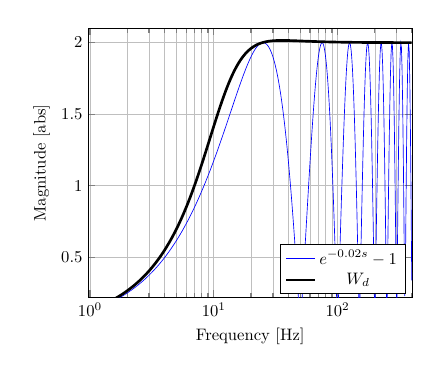
\begin{tikzpicture}[scale=0.6]
\begin{semilogxaxis}[%
legend style={at={(0.98,0.2)}},
no markers,
grid=both,
domain=1:400,
ymin=0.220,
ymax=2.1,
xmax=400,
samples=500,
tick style={thick},
xlabel=Frequency {[Hz]},
ylabel=Magnitude {[abs]}]
\addplot{sqrt(((-1+cos(0.02*deg(2*pi*x)))^2 + (sin(0.02*deg(2*pi*x)))^2)};
\addplot[ultra thick]
    {sqrt(((1600*pi^2*x^2 + 1)*(10000*pi^2*x^2 + 10387729))/(2500*(1600*pi^4*x^4 + 1028164*pi^2*x^2 + 3805656100))};
\legend{$e^{-0.02s}-1$,$W_d$}
\end{semilogxaxis}
\end{tikzpicture}
\phantomsubcaption\label{fig:delayvsW}%
\end{subfigure}
\caption[(a) Loop transformation for assuring $\tilde{\Delta}(0)=0$. (b) Frequency domain covering of the shifted delay 
operator.]{(a) Rewriting the interconnection such that $\tau=0$ implies 
$\tilde{\Delta}=0$. (b) Frequency domain covering of the shifted delay 
operator.}
\label{fig:3}
\end{figure}

The uncertainty is then characterized by using two properties of $\tilde \Delta$: For all 
$\omega,\tau$, the complex number $z=e^{-\iw{\tau}}-1$ is located on the unit circle centered 
at $(-1,0)$ in the complex plane. Since condition $\abs{z+1}=1$ translates into $z^*z+z^*+z=0$, 
we infer for all bounded $\Omega:\Real\to\Real$ that
\begin{equation}
\pmatr{\tilde{\Delta}(\iw)\\1}^*\pmatr{\Omega(\omega) &\Omega(\omega)\\ \Omega(\omega) &0}
\pmatr{\tilde{\Delta}(\iw)\\1} = 0\ \ \forall\omega\in\Real
\label{eq:onthecircle}
\end{equation}
for any delay time $\tau\in\Real$. Furthermore, we need to take the low frequency property of the 
magnitude of the frequency response into account. This is typically captured by a frequency dependent 
weight. If we define,
\begin{equation*}
W_d(s)= 2\frac{(s+ \frac{4}{\pi\bar{\tau}}) (s+ \frac{\beta}{\bar{\tau}})}%
{(s-\frac{\pi}{2\bar{\tau}}e^{i\theta})(s-\frac{\pi}{2\bar{\tau}}e^{-i\theta})}
\end{equation*}
with $\theta=\left( \frac{\pi}{2}\right)^2$ and some small $\beta>0$, then $W_d$ covers the delay 
uncertainty in the sense that $|\tilde{\Delta}(\iw)|\leq |W(\iw)|$ for all $\omega\in\Real$ and 
for all $\tau\in [0,\bar{\tau}]$. An example of magnitude covering is shown in \Cref{fig:delayvsW}.

This property, in turn, translates into $(\tilde{\Delta})^*\tilde{\Delta}\leq (W_d)^*W_d$ for all 
$\omega\in\Real$. Then we can utilize the classical $D$-scalings to obtain the following constraint 
with a dynamic multiplier:
\begin{equation}
\pmatr{\star}^*\pmatr{-\mathcal{D}(\omega) &0\\0 &W_d(\iw)^*\mathcal{D}(\omega)W_d(\iw)}
\pmatr{\tilde{\Delta}(\iw)\\1} \geq 0
\label{eq:normbounded}
\end{equation}
for all bounded $\mathcal{D}:\Real\to (0,\infty)$. Then the overall multiplier family results from a 
conic combination of \eqref{eq:onthecircle} and \eqref{eq:normbounded}:
\[
\pmatr{\star}^*\pmatr{-\mathcal{D}+\Omega &\Omega\\
\Omega &W_d^*\mathcal{D}W_d}\pmatr{\tilde{\Delta}\\1}
\geq 0 \quad \forall\omega\in\Real_e
\]

\section{Equivalent IQC Based Stability Tests for Common Stability Analysis Approaches}
\subsection{Llewellyn's Stability Criteria}\label{sec:ana:llewellyn}
%The well known conditions for stability of a two-port network, formulated in \cite{llewellyn,bolinder,rollett}, are recalled in the following theorem. An explicit indication of the frequency dependence is  {often} omitted for notational convenience.
%\begin{thm}[Unconditional Stability]\label{thm:llw}
%A $2$-port network $N$,  described by its transfer matrix
%\[
%N(\iw) = \pmatr{N_{11}(\iw) &N_{12}(\iw)\\N_{21}(\iw) &N_{22}(\iw)}
%\]
%and interconnected to passive termination immittances as in \Cref{fig:nom_net}, is stable if and only if
%\begin{equation}R_{11} > 0\text{ or } R_{22} > 0,\label{eq:llew2}\end{equation}
%\vspace{0ex}
%and
%\begin{multline}4\left(R_{11}R_{22}+X_{12}X_{21}\right)\left(R_{11}R_{22}-R_{12}R_{21}\right)\\-
	%\left(R_{12}X_{21}-R_{21}X_{12}\right)^2 > 0\label{eq:llew3}\end{multline} or
%\begin{equation}2R_{11}R_{22}-\abs{N_{12}N_{21}}-\Re{N_{12}N_{21}} > 0\tag{\ref{eq:llew3}$'$}\label{eq:llew3p}\end{equation}
%for all $\omega\in\Realext$, where $R_{ij}$ and $X_{ij}$ denote the real and imaginary parts of $N_{ij}$ respectively.
%\end{thm}
%
%\begin{rem}\label{rem:nonstrictness}In contrast to some references, this 
%result is formulated with strict inequalities in order to
%guarantee $\mathcal{L}_2$-gain stability (See also \cite[Sec. V]{lawrence}
%and \cite[Thm. 6.1]{khalil}).
%\end{rem}

As shown in \cite{rollett}, the conditions stated in \Cref{thm:apdx:llw} are invariant under
immittance substitution. Hence, we assume that the network and the terminations are represented
with an input/output mapping as depicted in  \Cref{fig:uncicpas}.

The stability conditions of \Cref{thm:apdx:llw} can be reproduced via the IQC theorem as 
follows. If $\Delta_l$ and $\Delta_s$ are passive and stable LTI systems, they satisfy
\[
\Delta_l + \Delta_l^* \geq 0 \ \ \text{and}\ \
\Delta_s + \Delta_s^* \geq 0
\]
for all $\omega\in\Realext$. If we choose arbitrary $\lambda_1(\omega)>0$ and $\lambda_2(\omega)>0$, it is clear that
the inequalities
$\lambda_2(\Delta_l + \Delta_l^*) \geq 0$ and $\lambda_1(\Delta_s + \Delta_s^*) \geq 0$
persist to hold, which can, in turn, be combined into
\[%\arraycolsep0.3ex
\pmatr{\Delta_s &0\\0 &\Delta_l\\\hline 1 &0\\0 &1}^*\left(\begin{array}{cc|cc}
      0&0  &\lambda_1 &0 \\
      0&0  &0         &\lambda_2\\ \hline
      \lambda_1 &0 &0 &0\\
      0 &\lambda_2 &0 &0
\end{array}\right)
\pmatr{\Delta_s &0\\0 &\Delta_l\\\hline 1 &0\\0 &1}
\succeq 0.
\]
After division by $\lambda_2(\omega)$ and with
$\lambda(\omega)=\frac{\lambda_1(\omega)}{\lambda_2(\omega)}$ we
obtain
\begin{equation}
\pmatr{\Delta_s &0\\0 &\Delta_l\\\hline 1 &0\\0 &1}^*\left(\begin{array}{cc|cc}
      0&0  &\lambda &0 \\
      0&0  &0         &1\\ \hline
      \lambda &0 &0 &0\\
      0 &1 &0 &0
\end{array}\right)
\pmatr{\Delta_s &0\\0 &\Delta_l\\\hline 1 &0\\0 &1} \succeq 0.
\label{eq:qcdeltall}
\end{equation}
In this fashion we have constructed a whole family of multipliers, parameterized by $\lambda(\omega)>0$, such that the quadratic constraint (\ref{eq:qcdeltall}) holds for all passive $\Delta_l,\Delta_s\in\mathcal{RH}_\infty$. Stability of the $N-\Delta$ interconnection is then guaranteed if one can find a positive $\lambda(\omega)$ for which the frequency domain inequality
\begin{equation}
\pmatr{1 &0\\0 &1\\\hline-N_{11} &-N_{12}\\-N_{21} &-N_{22}}^*
\left(\begin{array}{cc|cc}
      0&0  &\lambda &0 \\
      0&0  &0         &1\\ \hline
      \lambda &0 &0 &0\\
      0 &1 &0 &0
\end{array}\right)
\pmatr{1 &0\\0 &1\\\hline-N_{11} &-N_{12}\\-N_{21} &-N_{22}} \prec 0
\label{eq:LlewellynFDI}
\end{equation}
is also satisfied at each frequency $\omega\in\Realext$ (Negation of $N$ 
results from the application of the IQC theorem to the negative feedback 
interconnection \Cref{fig:uncicpas}). The resulting condition is equivalent 
to checking whether, at each frequency, there exists a $\lambda > 0$ such that
\[
H = \left[
\begin{array}{cc} - 2\lambda R_{11} &  -\lambda N_{12} - N^*_{21}\\ 
-\lambda N_{12}^* - N_{21} &-2R_{22} 
\end{array}
\right]\prec 0
\]
holds. This leads us to the relation with the classical results. Indeed, 
the $2\times 2$ matrix $H$ is negative definite if and only if
\[
R_{11} > 0 \quad \text{or} \quad R_{22} > 0
%\label{eq:llewellynaux}
\]
and
\[
\det H =  \left(-R_{12}^2 - X_{12}^2\right)\lambda^2 - R_{21}^2 - X_{21}^2 + \left(4R_{11}R_{22} - 2R_{12}R_{21} + 2X_{12}X_{21}\right)\lambda  > 0.
\]
Since the leading and constant coefficient of the involved polynomial are negative, 
the apex of the corresponding parabola should stay above the $\lambda$-axis. Using 
the apex coordinates of a concave parabola one can show that this is equivalent to 
\eqref{eq:lit:llew3}. Symmetry of the resulting conditions with respect to the indices 
is shown by simply switching the roles of $\lambda_1$ and $\lambda_2$ in our derivation.


\begin{rem} In the previous FDI condition \eqref{eq:LlewellynFDI} and if assuming 
$\lambda = 1$ over all frequencies, we also recover the Raisbeck's conditions 
\cite{raisbeck}. A comparison of Raisbeck's and Llewellyn's criteria indicates that 
the use of frequency dependent multipliers demonstrates the possibility of a substantial 
decrease of conservatism in stability analysis. In fact, the difference between Llewellyn's 
conditions and of Raisbeck's is the use of dynamic multipliers instead of static ones.
\end{rem}
\begin{rem} One should also note that Llewellyn's original conditions are both sufficient
and necessary and, hence, involve no conservatism. Exactness is due to the vast generality 
of the uncertainties, since one just assumes that the human and the environment are  
represented by passive LTI operators. The Nyquist curves of the corresponding positive 
real functions are only constrained {to be} lying in the closed right half plane. In 
reality, however, one is rather interested in operators whose Nyquist curves are confined 
to a sub-region of the closed right-half plane (or even to other bounded sets elsewhere 
in the complex plane). Covering the relevant region of interest in the complex plane 
with the full closed right-half plane for describing the involved uncertainty provides a 
clear account of the conservatism of the stability tests in teleoperation systems. Thus, 
if one wishes to reduce conservatism, additional structural information about the operators 
should be included {in order} to further constrain the uncertainty set (e.g. \cite{chopark,
hzaadsalcu,haddadizaad,willaertIJRR10}). It will be illustrated in \Cref{sec:num} how this 
can be achieved by using conic combinations of different multipliers which express refined 
properties of the involved operators.
\end{rem}

%===================================================================================
%===================================================================================
\subsection{Unconditional Stability Analysis of 3-port Networks}\label{sec:threeport}
For the analysis of 3-port networks, there exists no obvious unconditional stability 
result other than terminating one of the ports with a known environment model 
and then performing an analysis on the resulting 2-port network (see e.g. \cite{khademian} 
and references therein). Still, we can obtain the exact conditions for a 3-port case in a 
straightforward fashion along the above described lines without port termination. 
However, as expected, the test derived in this section is more conservative
than those of port termination based methods since the additional information about
the model with which the port is terminated renders the uncertainty set
significantly smaller.


If compared to the previous section, the only modification is to take a system 
representation $N\in\mathcal{RH}_\infty^{3\times 3}$ and three passive uncertainty 
blocks living in $\mathcal{RH}_\infty$ which are collected as
\begin{equation}
\Delta(\iw) = \text{diag} \left( \Delta_1(\iw),\Delta_2(\iw),\Delta_3(\iw)\right)
\label{eq:diagDelta}
\end{equation}
in order to model the three port terminations. With
\begin{equation}
\Lambda(\iw) = \text{diag}\left( \lambda_1(\omega),\lambda_2(\omega),\lambda_3(\omega)\right)\succ 0
\label{eq:diagLambda}
\end{equation}
we obtain the following quadratic constraint
\[
%\arraycolsep0.3ex
\pmatr{\Delta\\I}^*\pmatr{0 &\Lambda\\\Lambda &0}\pmatr{\Delta\\I}\succeq 0
%\label{eq:thportIQC}
\]
which reflects passivity of the three sub-blocks. The corresponding FDI for guaranteeing stability reads as
\begin{equation}
\pmatr{I \\ -N}^*
\pmatr{0 &\Lambda\\\Lambda &0}
\pmatr{I \\ -N} \prec 0.
\label{eq:thportFDI}
\end{equation}
%We arrive at the following 3-port unconditional stability condition.
\begin{thm}[Llewellyn's $3$-port Criteria]\label{thm:3portll}

A network, represented by its $3\times3$ transfer function $N \in \mathcal{RH}_\infty^{3\times 3}$ 
and in\-ter\-connected to the {stable}, passive and block diagonal $\Delta$ as given in 
\eqref{eq:diagDelta} is stable if and only if there exists a structured $\Lambda$ with 
\eqref{eq:diagLambda} such that \eqref{eq:thportFDI} holds for all $\omega\in\Realext$.
\end{thm}

Exact conditions for unconditional stability could be obtained  from \eqref{eq:thportFDI} 
by symbolic computations. However, getting formulas similar to {those in} \eqref{eq:lit:llew2}, 
\eqref{eq:lit:llew3} would lead to quite cumbersome expressions (see e.g. \cite{kuochu, tan, 
khademian}). Moreover, variants of expressing negative definiteness would result in different 
formulations of the stability conditions in terms of scalar inequalities. In the IQC formulation 
this is completely avoided while it is still possible to easily verify the resulting conditions 
numerically.


%===================================================================================
%===================================================================================
\subsection{Rollett's Stability Condition}\label{sec:rollett}
With almost identical arguments as for Llewellyn's test, 
one derives the following quadratic constraints {for positive $\lambda$} and for stable LTI systems 
$\tilde{\Delta}_l$ and $\tilde{\Delta}_s$ whose gains are bounded by one:
\[
\pmatr{\tilde{\Delta}_s &0\\0 &\tilde{\Delta}_l\\\hline 1 &0\\0 &1}^*\left(\begin{array}{cc|cc}
-\lambda  &0  & 				& \\
0	  			&-1  &  				&\\ \hline
	  			& 	&\lambda 	&0\\
	  			& 	&0 				&1
	  			\end{array}\right)
\pmatr{\tilde{\Delta}_s &0\\0 &\tilde{\Delta}_l\\\hline 1 &0\\0 &1} \succeq 0.
\]

Interconnection stability is then assured if one can find a positive frequency dependent 
$\lambda$ for which the FDI
\begin{equation}
\pmatr{1 &0\\0 &1\\\hline S_{11} &S_{12}\\S_{21} &S_{22}}^*\left(\begin{array}{cc|cc}
-\lambda  &0  & 				& \\
0	  			&-1  &  				&\\ \hline
	  			& 	&\lambda 	&0\\
	  			& 	&0 				&1
\end{array}\right)
\pmatr{1 &0\\0 &1\\\hline S_{11} &S_{12}\\S_{21} &S_{22}} \prec 0
\label{eq:rolFDI}
\end{equation}
or, equivalently,
\[
H = \bmatr{\abs{S_{21}}^2 + \lambda(\abs{S_{11}}^2 - 1) &S_{22}S_{21}^* + \lambda S_{12}S_{11}^*\\
S_{22}^*S_{21} + \lambda S_{12}^*S_{11} &\abs{S_{22}}^2 - 1 + \lambda\abs{S_{12}}^2 }\prec 0
\]
hold for all $\omega\in\Realext$. Then, it is elementary to express $H\prec0$ by $\det{({H})}>0$ 
and by negativity of the diagonal entries of $H$ for all $\omega\in\Realext$. Positivity of the 
determinant of $H$ means
\[
(1- \abs{S_{22}}^2 - \abs{S_{11}}^2 +\abs{\nabla}^2)\lambda - \abs{S_{12}}^2\lambda^2 - \abs{S_{21}}^2 > 0.
\]
If this is expressed as $f(\lambda)= -a\lambda^2+b\lambda-c>0$ with $a,c>0$, we require the 
apex coordinates $\smash{\left(\frac{b}{2a},\frac{b^2-4ac}{4a}\right)}$ both to be positive. 
Since $a>0$, we have
\begin{equation}
(1+\abs{\nabla}^2 - \abs{S_{22}}^2 - \abs{S_{11}}^2)^2 > 4\abs{S_{12}S_{21}}^2
\label{eq:prerollett1}
\end{equation}
due to $b^2>4ac$. Moreover, negativity of the diagonal terms {is expressed as}
\begin{equation}\label{eq:prerollett2}
\lambda(1-\abs{S_{11}}^2) > \abs{S_{21}}^2 \quad \text{or} \quad 1- \abs{S_{22}}^2 > \lambda\abs{S_{12}}^2.
\end{equation}
To make the connection to the classical auxiliary conditions, observe that evaluating 
$f(\lambda)$ at  $\lambda_0=\sqrt{\frac{c}{a}} =\tfrac{\abs{S_{21}}}{\abs{S_{12}}}$ would 
lead to the condition $b>0$ since $f(\lambda_0)=b\sqrt{\frac{c}{a}}-2c>0$. Hence 
\eqref{eq:prerollett2} becomes
\begin{equation}
1-\abs{S_{11}}^2 > \abs{S_{12}S_{21}} \quad \text{or} \quad 1- \abs{S_{22}}^2 > \abs{S_{12}S_{21}}.
\label{eq:rollettaux}
\end{equation}
{In the literature, the quantity $\lambda_0$ is called the ``maximum stable power gain".} Finally, 
after explicitly including the condition $b>0$, one can take the square root of \eqref{eq:prerollett1} 
and obtain
\[
1+\abs{\nabla}^2 - \abs{S_{22}}^2 - \abs{S_{11}}^2 > 2\abs{S_{12}S_{21}},
%\label{eq:rollett1}
\]
which is precisely Rollett's first condition.

There has been quite some discussion in various studies (e.g. \cite{lombardi,edsin,woods,pirola}) 
whether testing both conditions in \eqref{eq:rollettaux} is really required, while it rolls out 
from our FDI arguments that one of these auxiliary inequalities is sufficient. In fact, 
\eqref{eq:rolFDI} renders this discussion obsolete since we deal with a single matrix inequality 
to be tested at each frequency. This test is equivalent to the one based on the Edwards-Sinsky 
stability parameter $\mu$ (\cite{edsin}) in the sense that only one condition needs to be verified. 
Alternatively, one can perform a symbolic computation of the largest eigenvalue of $H$ and search 
for a positive $\lambda$ that renders that quantity strictly negative. Recently, the $\mu$ parameter 
has been used in the context of teleoperation in \cite{haddadizaad} and their results can also be 
recovered by using multipliers similar to the ones given in the next section.

%===================================================================================
%===================================================================================
\begin{figure}
\begin{center}
\begin{tikzpicture}[>=stealth,scale=0.75,transform shape,every node/.style={minimum height=1.1cm,minimum width=1.1cm},label distance=1mm]
\node[draw] (del) at (-3,2) {$\frac{1-e^{-s\tau}}{s} $};
\node[draw] (plant) at (0,2) {$\frac{1}{ms+b}$};
\node[draw] (integ) at (3,2) {$\frac{1}{s}$};
\node[draw] (z0) at (0,3.5) {$Z_0$};
\node[draw,label={[text width=1.6cm,inner sep=0,scale=0.8,xshift=1mm,yshift=2mm]below:{\small Unilateral Constraint}}] (uniconst) at (1,0) {\tikz{
\draw[thick,->] (0.5,0)--(0.5,1);\draw (0.5,0.5) -- (1,1);\draw[thick,->] (0,0.5) -- (1,0.5);}
};
\node[draw] (h) at (-1.5,0) {$H(z)$};
\node[circle,minimum size=0mm,inner sep=1mm,draw,%
label={[minimum size=0mm,inner sep=0mm]100:$-$},
label={[minimum size=0mm,inner sep=0mm]175:$-$}] (j) at ($(del.east)!0.5!(plant.west)$) {};
\draw[->] (plant.east) -- (integ.west);
\draw[->]  (integ.east) -| ++(0.5,-0.5) |- (3.5,0) -- ($(3.5,0)!1!-40:++(-0.5,0)$) node[anchor=north,inner sep=0] {$T$} (3,0) -- (uniconst.east);
\draw[->] (uniconst.west) -- (h.east);
\draw[->] (h.west) -| ($(del.west)-(0.5,0)$) -- (del.west);
\draw[->] (del.east) -- (j.west);
\draw[->] (j.east) -- (plant.west);
\draw[->] ($(plant.east)!0.5!(integ.west)$) |- (z0.east);
\draw[->] (z0.west) -| (j.north);
\end{tikzpicture}
	\caption{The teleoperation setup from \cite{colgate1}}
	\label{fig:colgate}
\end{center}
\end{figure}
\subsection{Colgate's Minimum Damping Condition}\label{sec:colgate}

In this section, the analysis problem from \cite{colgate2,colgate3} is investigated by IQCs. 
In this example, the master device {is} modeled as $\frac{1}{ms+b}$ {and} is combined with 
a passive operator impedance $Z_0(s)$ {as shown in} \Cref{fig:colgate}. We limit the 
analysis to the {situation} without the unilateral constraint. The overall operator and master 
device transfer function reads as $\Delta(s) = \frac{1}{ms+b+Z_0(s)}$. Since $Z_0(s)$ is 
passive and $b$ {is positive}, the Nyquist curve of $\Delta^{-1}(s)$ is confined to the 
half-plane $\{z\in\mathbb{C}: \Re{z} \geq b\}$ {and $\Delta^{-1}(s)$ is strictly input 
passive with parameter $b$.} In \cite{colgate2}, the problem is converted to the small 
gain theorem with a geometric reasoning. In our setting, passivity is expressed as
\[
\pmatr{1\\ \Delta(\iw)^{-1} }^*
\pmatr{-2b &1\\1 &0}
\pmatr{1\\ \Delta(\iw)^{-1} } \geq 0
\]
which is clearly equivalent to
\[
\pmatr{\Delta(\iw)\\ 1 }^*\pmatr{-2b &1\\1 &0}\pmatr{\Delta(\iw)\\1} \geq 0
\]
for all $\omega\in\Realext$. The FDI guaranteeing stability then reads as
\[
\pmatr{1\\ -G_d(\iw)}^*\pmatr{-2b &1\\1 &0}\pmatr{1\\ -G_d(\iw)} < 0
\]
for all $\omega\in\Realext$. Using the closed form formula in \cite{colgate2},
\begin{equation*}
G_d(\iw) = \frac{T}{2}\frac{e^{\iw T}-1}{1- \cos{(\omega T)}}H(e^{\iw T}),
%\label{eq:Colgateclosedform}
\end{equation*}
this directly leads to Colgate's original condition:
\begin{multline*}%\label{eq:colgate}
-2b - G_d^*(\iw) - G_d(\iw) < 0 \\
\Longleftrightarrow b > \frac{T}{2}\frac{1}{1-\cos{(\omega T)}}\Re{(1-e^{-\iw T})H({e^{\iw T}})}.
\end{multline*}
{The employed multiplier can be transformed into the one for the small-gain theorem along the following lines:}
\begin{align*}
0&\leq  2b\pmatr{\Delta(\iw)\\ 1 }^*\pmatr{-2b &1\\1 &0}\pmatr{\Delta(\iw)\\1} \\\nonumber  %\label{eq:dummymult}
&=\pmatr{\Delta(\iw)\\1}^*\left[\pmatr{2b&-1\\0&1}^T\pmatr{-1 &0\\0 &1}\pmatr{2b&-1\\0&1}\right]\pmatr{\Delta(\iw)\\1}\\\nonumber
&=\pmatr{2b\Delta(\iw) - 1\\ 1 }^*\pmatr{-1 &0\\0 &1}\pmatr{2b\Delta(\iw) - 1\\ 1 } \Longleftrightarrow |2b\Delta(\iw)-1| \leq 1.
\end{align*}
This links our arguments to those appearing in \cite{colgate2,colgate3} and reveals that the direct application of 
tools from robust control allows to circumvent any transformation to scattering parameters (or, in other words, 
the application of a loop transformation) for obtaining the stability conditions. In fact, the congruence transformation
\begin{equation*}\arraycolsep0.5ex
%\label{eq:scat}
\left(\frac{1}{\sqrt{2b}}\pmatr{1 &-b\\1&b}\right)^T\pmatr{-1 &0\\0
&1}
\left(\frac{1}{\sqrt{2b}}\pmatr{1 &-b\\1 &b}\right) = \pmatr{0&1 \\
1 &0}
\end{equation*}
with the scattering transformation matrix turns the small-gain multiplier into the one for passivity. This observation 
allows to easily show the equivalence of the small gain and passivity theorems through scattering transformations 
(\cite{andersonspong}) and wave variable methods (\cite{nieslotine,nieslotine2}).

%===================================================================================
\subsection{Regions in the Complex Plane}
Using a similar mechanism to what is given above, one can also characterize other domains in the complex 
plane different than the whole right half plane as long as it can be represented (or covered with) with a 
quadratic constraint. Thus, once a multiplier family is set, it's a matter of evaluating the respective FDI for the system
at hand. For example, recently in \cite{jazayeri}, a vertical strip-like domain for one of the LTI uncertainties is 
assumed i.e. $-a\leq \Delta_l + \Delta_l^* \leq b$ for all $\omega\in\Real_e$ with $a,b>0$ 
and stability conditions are derived similar to those of Llewellyn's test along the lines of \cite{edsin}. In terms of quadratic 
constraints, a direct verification of the constraints below 
\[
\pmatr{\Delta(\iw)\\ 1 }^*
\pmatr{0 &1\\1 &a}
\pmatr{\Delta(\iw)\\ 1 } \geq 0 \text{ and }
\pmatr{\Delta(\iw)\\ 1 }^*
\pmatr{0 &-1\\-1 &b}
\pmatr{\Delta(\iw)\\ 1 } \geq 0
\]
show that these constraints characterize the domain 
\[
\{z\in\mathbb{C}: -a \leq \Re{z} \leq b \text{ for }a,b>0\}.
\]
Hence, via introducing dynamic multipliers and scaling the overall multiplier with the corresponding $\lambda$ of $\Delta_s$,
the stability condition is equivalent to, for each $\omega\in\Real_e$ the existence of $\lambda_1(\omega),\lambda_2(\omega)>0$ 
such that
\begin{equation}
\pmatr{1 &0\\0 &1\\\hline-N_{11} &-N_{12}\\-N_{21} &-N_{22}}^*
\left(\begin{array}{cc|cc}
      0 &0                   &1 &0                  \\
      0 &0                   &0 &\lambda_1-\lambda_2\\ \hline
      1 &0                   &0 &0                  \\
      0 &\lambda_1-\lambda_2 &0 &\lambda_1 a+\lambda_2 b
\end{array}\right)
\pmatr{1 &0\\0 &1\\\hline-N_{11} &-N_{12}\\-N_{21} &-N_{22}} \prec 0
\label{eq:jazayeritest}
\end{equation}
holds. By carrying out the multiplication, we obtain 
\[
\pmatr{
-2R_{11} + (\lambda_1 a+\lambda_2 b)\abs{N_{21}}^2 & -N_{12} -(\lambda_1 -\lambda_2)N_{21}^*+(\lambda_1 a+\lambda_2 b)N_{21}^*N_{22}\\
\star                                              &-2(\lambda_1 -\lambda_2)R_{22}+(\lambda_1 a+\lambda_2 b)\abs{N_{22}}^2
}\prec 0.
\]
%\[
%\pmatr{
%-2R_{11} + \lambda_1 a\abs{N_{21}}^2 & -N_{12} -(\lambda_1 -\lambda_2)N_{21}^*+\lambda_1 aN_{21}^*N_{22}\\
%\star                                              &-2(\lambda_1 -\lambda_2)R_{22}+\lambda_1 a\abs{N_{22}}^2
%}\prec
%\lambda_2 b
%\pmatr{
%N_{21}^*\\N_{22}^*
%}
%\pmatr{
%N_{21}^*\\N_{22}^*
%}^*.
%\]

%If we compare this with the derived conditions in \cite{jazayeri}, we can see that their results don't involve any $b$ terms. Hence, 
%contrary to the claim, those results can be, at best, sufficient since their test only deals with the first part of the constraint, namely 
%$-a\leq \operatorname{Re}({\Delta_l})$. Still we cannot see the actual problematic step as we cannot reproduce their conditions by leaving out 
%the constraint involving $b$ term. Nevertheless, their first remark in \cite[Theorem 3]{jazayeri} is not correct. The upper bound 
%on the real part of the uncertainty certainly plays a role and can not be omitted in the necessity direction in their proof which is omitted 
%in their paper. In other words two uncertainty operators with $\operatorname{Re}{\Delta}\leq b (\geq b)$ for some frequencies respectively,
%can not be distinguished and this possibility already contradicts with the necessity of the test since both will be evaluated on the 
%basis of parameter $a$ and regardless of $b$. 

If compared to the results of \cite{jazayeri}, terms involving the bound $b$ don't vanish. In fact, the authors prove the 
test for a half-plane defined as $\left\{z\in\Complex|\Re{z}\geq a\right\}$ instead of a strip and the necessity direction 
of the proof is omitted. Hence, the upper bound on the real part of the uncertainty is not taken into account. Thus, their 
result is similar to the condition given in \Cref{thm:desvidpass}. In fact it becomes more visible if we separate the terms
in \eqref{eq:jazayeritest} as the following:
\[
\pmatr{\star}^*
\left(\begin{array}{cc|cc}
      0 &0                   &1 &0                  \\
      0 &0                   &0 &\lambda_3\\ \hline
      1 &0                   &0 &0                  \\
      0 &\lambda_3           &0 &\lambda_3 a
\end{array}\right)
\pmatr{I\\\hline-N} \prec
-(a+b)\lambda_2
\pmatr{N_{21}^*\\N_{22}^*}
\pmatr{N_{21} &N_{22}},
\]
where we impose $\lambda_3\coloneqq \lambda_1 - \lambda_2 > 0$ for all frequencies since for each positive $\lambda_3$ we can find
a $\lambda_1$ such that the inequality is satisfied. One can show that the left hand side is precisely the authors condition. Also
the right hand side is a negative semidefinite perturbation that pushes the left hand side more into negative definiteness. Notice 
that this condition, as the authors also remark, shows that $b$ term can be arbitrarily large. It is a matter of choosing $\lambda_2$ 
sufficiently small to render the inequalities feasible. In fact having $b\to\infty$ implies $\lambda_2\to 0$. Hence rendering the 
second constraint above useless. The reason for the absence of $b$ terms in \cite{jazayeri} is due to the incorrect formulation of 
Llewellyn's stability theorem with nonstrict inequalities. Obviously it is not a major obstacle however as seen here it leads to wrong
inferences about asymptotical stability. 


In summary, having an upper bound on the real part of the impedance is not a structurally important modeling issue. Though in case of
an unstructured uncertainty the conditions are indeed sufficient and necessary, we also see that our modeling approach is still
conservative and including the $b$ bound doesn't bring in any specialization in terms of the conditions. In other words, it doesn't 
matter if $b$ is very small or very large. Thus, it does not offer any improvement.


\begin{rem}
In \cite{jazayeri}, the results above are presented as novel stability conditions, but essentially, they are the reformulations of 
the general passivity theorem that can be found elsewhere. This formulation is also equivalent to \cite{haddadizaad} which also uses 
the M\"{o}bius transformation arguments given by \cite{edsin}\footnote{In fact, \cite{edsin,lombardi} further include an argument and 
a correction about often cited but erroneous version of absolute stability theorem as we have replicated in IQC version above. For some 
reason, the nonstrict version given in \cite{haykin}, which is not accurate, is persistently being cited even when Llewelyn's original
paper is cited.} up to scattering transformations which once again in turn equivalent to the formulation given above. Alternatively, 
\cite{hirchebuss} gives another reformulation using $QSR$-dissipativity which is the case of having static multipliers in our examples, 
which in turn another manifestation of \cite[Thm. 6.2]{khalil} for non-LTI end terminations. 

This is just another instance of our main argument; had the problem been formulated as a straightforward robustness test, 
it would have been relatively easy to see the connection with the classical results. However, since the problem formulation is given 
in a network theory context, any stability result that is not present in network theory is claimed to be original which is regrettably 
incorrect. The teleoperation literature should be synced with the systems theory literature to avoid doubling the efforts. This also 
applies to IQCs that if there exists a better tool out there which surpasses the convenience and generality of IQC framework then use 
of IQCs should be avoided. The point we wish to make is that none of the methods are essential in the solution of the bilateral 
teleoperation problem and thus there is no reason to insist on a certain way of looking at the problem.
\end{rem}


Note that, we can take not just rectangles or circles but any arbitrary path connected region as long as we can describe 
the constraints with quadratic forms. Therefore the methodology is significantly general than merely dealing with active/passive
uncertainty modeling. As a trivial example, we can cover/overbound the uncertainty region with an ellipsoid which in turn leads to
a quite substantial improvement over the passivity case since then the constraint type will not be a positive realness test and 
yet the uncertainty set would be significantly smaller. Hence more potential for improvement. Another example is given above in the 
delay multiplier construction. We can also combine inequality/equality constraints to further restrict the robustness test in
order to reduce conservatism. 

Moreover, as is the case for the previous examples, one can impose the constraints above and possibly more on both the human 
and the environment uncertainties, without invoking the passivity theorem explicitly, in a few steps instead of deriving 
standalone conditions for each individual case with rather cumbersome manipulations. 

%===================================================================================
\subsection{Exactness of Robustness Tests}\label{sec:exact}
As mentioned before, IQC-based stability criteria are typically only sufficient.
Still the classical conditions as discussed above %in Sections \ref{sec:llewellyn} to \ref{sec:colgate}
turn out to be also necessary. Necessity of these criteria can as well be seen to be a specialization of
celebrated exactness results in structured singular-value theory. In fact, IQC tests
for structured LTI uncertainties with two or three full diagonal blocks as derived above are known to be always exact.
This implies, in particular, that the 3-port counterpart of Llewellyn's conditions is indeed
a necessary and sufficient test for stability. It's not feasible for us to provide a full treatment of all possible 
cases in which IQC-based robustness tests are known to be exact. Nevertheless, for a detailed discussion related to LTI 
uncertainties we refer to \cite{packdoyle,fantits,cwssimax}.

We would like to emphasize that these beautiful exactness properties come at the price of some limitations 
of the classical framework. For instance, Llewellyn's conditions are not sufficient for stability any more 
if we only assume that the uncertainties are passive but not necessarily LTI. On the other hand, if allowing 
for arbitrary causal and passive uncertainties, stability is still guaranteed if we can find a 
frequency-independent $\lambda>0$ which renders the FDI \eqref{eq:LlewellynFDI} satisfied, and this property 
can be easily verified numerically.

%===================================================================================
\section{Numerical Case Studies}\label{sec:num}
In this section, we show how frequently encountered analysis problems can be solved 
under the IQC formulation with ease. We utilize the multipliers as given above for  
robustness tests applied to a simple teleoperation system taken from \cite{willaert,
willaertIJRR10}. Our main emphasis is on showing how one can reproduce the numerical 
results of such frequency domain techniques and 
how it is possible to substantially widen the range of allowed uncertainties in the 
IQC framework for which no classical analytical stability tests exist. This serves as 
an illustration for the possibility to improve analysis and, more importantly in 
future work, optimization-based controller synthesis results if better human/environment 
models become available.

\subsection{Algorithmic Verification}\label{sec:algver}

We have discussed some classical stability tests that reduce to explicit scalar 
inequalities which can be verified in a frequency-by-frequency fashion. In contrast, 
the equivalent re-formulations in terms of IQCs open the way to verifying these conditions 
numerically, by applying algorithms from the by now well-established area of semi-definite 
programming \cite{lmiboydbook}. For example, checking at each frequency the existence of 
some diagonal $\Lambda\succ 0$ which satisfies \eqref{eq:thportFDI} boils down to an 
efficiently tractable LMI problem in the three diagonal entries of $\Lambda$, which 
can be readily implemented in software environments such as \cite{yalmip}. We also 
show how it is even possible to avoid any frequency-gridding and to reduce the tests 
to finite-dimensional semi-definite programming problems that can be solved in one shot.

This section serves to illustrate this procedure for Rollett's stability condition, 
which requires to determine a frequency-dependent bounded and strictly positive 
$\lambda$ satisfying the FDI \eqref{eq:rolFDI}. Without loss of generality, it 
suffices to search for proper and rational functions $\lambda$ that have no poles 
and are positive on the extended imaginary axis. Due to the well-established spectral 
factorization theorem (e.g. \cite{francis}), we can express any such function as 
$\psi^*\psi$ with some stable transfer function $\psi$ (without zeros in the closed 
right half-plane). For some fixed pole $a<0$ let us choose the basis vectors
\begin{equation*}
\Phi_n(s) = \pmatr{1 &\frac{1}{s-a} &\frac{1}{(s-a)^2} &\cdots &\frac{1}{(s-a)^{n-1}}}^T
%\label{eq:outerfactor}
\end{equation*}
for $n=\mathbb{N}$. By a well-known fact from approximation theory (\cite{pinkus}), 
the function $\psi$ can be approximated to an arbitrary degree by $L^T\Phi_n$ for some 
suitable $L\in\Real^n$ uniformly on the imaginary axis, if only $n$ is taken sufficiently 
large. More precisely, $\inf_{L\in\Real^n}\|\psi-L^T\Phi_n\|_\infty$ converges to zero for 
$n\to\infty$. In summary, any proper rational $\lambda$ with $\lambda(\iw)>0$ for 
$\omega\in\Realext$ can be approximated arbitrarily closely by $\Phi_n^*LL^T\Phi_n$ or, 
in turn, by $\Phi_n^*D\Phi_n\text{\ \ with\ \ }D=D^T\in\Real^{n\times n}.$

This discussion justifies why one can parameterize the multiplier (middle term) in \eqref{eq:rolFDI} as
\[\arraycolsep0.3ex
\Psi_n^*
\underbrace{\left(\begin{array}{cc|cc}
-D&0  & 				& \\
0	  			&-1  &  				&\\ \hline
	  			& 	&D &0\\
	  			& 	&0 				&1
\end{array}\right)}_{M}
\underbrace{\left(\begin{array}{cc|cc}\Phi_n &&&\\ &1 &&\\\hline &&\Phi_n& \\&&&1\end{array}\right)}_{\Psi_n}
\]
in terms of a frequency-dependent outer factor $\Psi_n$ and a diagonally structured real 
symmetric matrix $M$ in the middle. Let us denote the set of all these matrices $M$ by 
$\mathcal{M}$ (dropping the dependence on $n$). For checking Rollet's condition we then need 
to verify the existence of $M\in{\mathcal{M}}$ such that the FDIs
\begin{equation*}
\Phi_n^*D\Phi_n>0\text{\ \ and\ \ }
\pmatr{I\\S}^*\Psi_n^*M\Psi_n\pmatr{I\\S} \prec 0
%\label{eq:rolFDI2}
\end{equation*}
are satisfied. We include the classical result (\cite{rantzerkyp}) that allows us to 
convert these frequency domain inequalities into LMIs:
\begin{thm}\label{KYP}[KYP Lemma] Let $G=\tikz[baseline={([yshift=-3pt]current bounding box.center)},
scale=0.8,transform shape]{\matrix (s1) [ssmatrix] {A \& B \\ C \& D \\};\draw (s1-1-1.north east) --
(s1-2-1.south east) (s1-1-1.south west) -- (s1-1-2.south east);}$ and suppose that $A$ has no eigenvalues on 
the imaginary axis. For a real matrix $P=P^T$, the following {two statements} are equivalent:
\begin{enumerate}
	\item The following FDI holds:
	\begin{equation}
	{G(\iw)}^*P {G(\iw)} \succ 0 \ \ \forall \omega\in\Realext.
	\label{eq:KYPFDI}
	\end{equation}
	\item There exists a symmetric matrix $X$ with
	\begin{equation}
	\pmatr{I &0\\A &B\\ \hline C &D}^T 
	\left(\begin{array}{cc|c}0 &X &0\\X &0 &0\\
	\hline 0 &0 &P\end{array}\right) 
	\pmatr{I &0\\A &B\\ \hline C &D} \succ 0.
	\label{eq:KYPLMI}
	\end{equation}
\end{enumerate}
\end{thm}

Now choose the minimal state space realizations
\begin{equation*}
\Phi_n = \left[ \begin{array}{c|c}
	A_{\Phi} &B_{\Phi}\\ \hline C_{\Phi} &D_{\Phi}
\end{array} \right]
\text{\ \ and\ \ }
\Psi_n\pmatr{I\\S} = \left[ \begin{array}{c|c}
	\mathcal{A} &\mathcal{B}\\ \hline \mathcal{C}&\mathcal{D}
\end{array} \right].%\label{outfac}
\end{equation*}
This allows to apply the KYP Lemma in order to equivalently convert $\lambda>0$ 
and \eqref{eq:rolFDI} into the feasibility of the LMIs
\begin{equation}
\pmatr{I &0\\A_{\Phi} &B_{\Phi}\\C_{\Phi}&D_{\Phi}}^T
\pmatr{0 &Z &0\\Z &0 &0\\0 &0 &D}
\pmatr{I &0\\A_{\Phi} &B_{\Phi}\\C_{\Phi}&D_{\Phi}} \succ 0
\label{eq:outerpos}
\end{equation}
and
\begin{equation}
\pmatr{I &0\\\mathcal{A} &\mathcal{B}\\\mathcal{C}&\mathcal{D}}^T
\pmatr{0 &\mathcal{X} &0\\ \mathcal{X}&0 &0\\0 &0 &M}
\pmatr{I &0\\\mathcal{A} &\mathcal{B}\\\mathcal{C}&\mathcal{D}} \prec 0.
\label{eq:KYPex}
\end{equation}
More precisely, if one can computationally verify the existence of $X$, $Z$, $M\in{\mathcal{M}}$
and $D=D^T$ which satisfy \eqref{eq:outerpos} and \eqref{eq:KYPex}, we have verified Rollet's
condition. Conversely, if Rollet's condition holds, then these LMIs are guaranteed to have
solutions if $n$ is chosen sufficiently large.

Let us emphasize again that the very same procedure applies to considerable more
complex interconnections and structured uncertainties $\Delta$. In fact, for many
interesting classes of uncertainties one can systematically construct multiplier
families (see e.g. \cite{megretski}) which are known to admit a description of the
form $\Pi = \Psi^*M\Psi,\ \ M\in\mathcal{M}$ with a stable outer factor transfer matrix
$\Psi$ and with some set of structured symmetric matrices ${\mathcal{M}}$ that can itself
be described as the feasible set of an LMI. Checking stability of the $G-\Delta$
interconnection in \Cref{fig:uncic} then requires to verify the validity of the FDI
\begin{equation*}
\pmatr{I\\G}^*\Psi^*{M}\Psi\pmatr{I\\G} \prec 0.
%\label{eq:IQCthmFDIfact}
\end{equation*}
Literally along the same lines as described above this is translated into a semi-definite 
program with Theorem \ref{KYP}.

\begin{rem}
In our numerical examples the basis length $n$ is chosen large enough that the performance level 
does not significantly change by further increasing $n$. As shown below, 
the required length $n$ for adequate accuracy in the multipler approximation
is (regardless of the conservatism of the test) often quite small in practice. 
\end{rem}

In what follows, we will continue to utilize the shorthand notation of
state-space realizations in a similar manner, i.e., $\mathcal{A,B,C,D}$ for
the combined outer factors by replacing $S$ with the respective plant, and
$A_\Phi,B_\Phi,C_\Phi,D_\Phi$ for the basis vector.


\subsection{System Model}
In \cite{willaert}, a simple teleoperation system described with the following equations is 
considered:
\begin{align*}
F_h+\tau_m &= M_m \ddot{x}_m + B_m \dot{x}_m\\
\tau_s -F_e &= M_s \ddot{x}_s + B_s \dot{x}_s.
\end{align*}
Here $M_m,M_s$ are the masses, $B_m,B_s$ are the damping coefficients, $\tau_m,\tau_s$ 
are the device motor torques, {and} $x_m,x_s$ are the position coordinates of the local 
and the remote devices respectively. $F_h,F_e$  denote the human and the environment forces. 
The human and the environment are assumed to be LTI passive operators {and} {are denoted by 
$\Delta_h,\Delta_e$ which substitute $\Delta_s,\Delta_l$ as employed in the more general 
network-related context in the earlier sections.}

Additionally, a particular PD type of a position-force controller scheme, denoted 
by \textbf{P}-\textbf{F} , is used:
\[
\tau_s = K_p(\mu x_m-x_s)-K_v \dot{x}_s ,\quad \tau_m = -K_f F_e.
\]
The overall teleoperation system is {then described}, with $Y_m(s) = \inv{(M_ms+B_m)}$ and 
$Y_s(s) = \frac{\mu K_p}{M_s s^2+(B_s+K_v)s+K_p}$, in terms of the following admittance matrix:
\begin{equation}
 Y = \pmatr{Y_m &- {K_f}Y_m\\ -Y_mY_s&\frac{M_m s^2+B_m s+\mu K_f K_p}{(M_s s^2+(B_s+K_v)s+K_p)}Y_m}.
\label{eq:admitsys}
\end{equation}
As shown in \cite{willaert}, the system's performance is related to the transparency of the 
teleoperator, {which is characterized by the maximal} attainable {product $\mu K_f$} while 
maintaining stability (see also \cite{danielmcaree}). We will evaluate our results with respect 
to this performance measure. For all computations, we have used \cite{sdpt3,sedumi,yalmip} 
with MATLAB 7.12.0 on a computer with a \SI{2.4}{\giga\hertz} processor and with 
\SI{4}{\giga\byte} RAM memory running Win 7-64 Bit OS. The system parameters are $M_m=0.64, 
M_s=0.61,B_m=0.64,B_s=11,K_v=87.8,K_p=4000$.

\begin{figure}
\begin{subfigure}[b]{.5\linewidth}
\centering%
	\begin{tikzpicture}[>=stealth,scale=0.7,transform shape]
	\matrix [draw,matrix of math nodes,nodes={transform shape,scale=0.7},ampersand replacement=\&] 
	(y) at (0,0) { Y_{11} \& Y_{12} \\ Y_{21} \&Y_{22} \\ };
	\matrix [draw,matrix of math nodes,nodes={transform shape,scale=0.7},ampersand replacement=\&] 
	(d) at (0,2cm) { \Delta_h \&\\ \&\Delta_e \\};
	\node[draw,circle,inner sep=2,label={180:$-$}] (junc) at (-1.5,1) {};
	\draw[->] (y.west) -| (junc.south);
	\draw[->] (junc.north) |- (d.west);
	\draw[->] (d.east) -| (1.5,1) |- (y.east);
	\end{tikzpicture}
\caption{Unconditional Stability}\label{fig:Case1blockdia}
\end{subfigure}%
\begin{subfigure}[b]{.5\linewidth}
\centering%
\begin{tikzpicture}[>=stealth,transform shape,scale=0.7]
\matrix [draw,matrix of math nodes,nodes={scale=0.7,transform shape},ampersand replacement=\&] 
(plant) at (0,0) { Y_{11} \& Y_{12} \\ Y_{21} \&Y_{22} \\ };
\matrix [draw,matrix of math nodes,nodes={scale=0.7,transform shape},ampersand replacement=\&] 
(del) at (0,2) { \Delta_h \\ \& \delta_e \\ };
\draw[->] (plant.160) -| ++ (-0.7,0.5) node[draw,circle,fill=white,inner sep=2,label=180:$-$] {} |- (del.160);
\draw[<-] (plant.20) -| ++ (0.7,0.4) |- (del.20);
\draw[->] (plant.-160) -| ++ (-0.3,0.5) |- (del.-160);
\draw[<-]  (plant.-20) -| ++ (0.3,0.4) |- (del.-20);
 \end{tikzpicture}
\caption{Uncertain stiff environment}\label{fig:Case2blockdia}
\end{subfigure}
\caption{System interconnections for \Cref{sec:numcase1} and \Cref{sec:numcase2}.}\label{fig:6}
\end{figure}


\subsection{Case 1 : Unconditional Stability Analysis via IQCs}\label{sec:numcase1}
We start with applying Llewellyn's test based on \eqref{eq:LlewellynFDI} to the system given 
above. In a first computation, we choose a frequency grid of $2000$ logarithmically spaced 
points in \SIrange{0}{10000}{\radian\per\second} and solve, at each grid point, 
a feasibility problem in $\lambda>0$. This is incorporated into a bisection algorithm that 
searches for the maximum value of $\mu K_f$ for which feasibility at each grid-point can be 
guaranteed. Due to gridding, this method typically gives an upper bound rather than the exact 
value on the guaranteed performance level, just because there is a chance to miss critical 
frequencies. Nevertheless, we obtained the exact value $\approx 0.137$ as in  \cite{willaert}. 
The inner search for $\lambda$ requires \SI{8.52}{\second}, while the overall computation 
takes about \SI{117}{\second}; note that the latter heavily depends on the initial bisection 
interval and on the desired accuracy.

In a second computation, we follow the path as described in \Cref{sec:algver}. The resulting FDI is
\begin{equation} \left(\Psi \pmatr{I\\-Y}\right)^* M
\left(\Psi \pmatr{I\\-Y}\right)\prec 0\label{eq:numcase1FDI}
\end{equation}
where
\begin{equation}
\arraycolsep0.3ex
\Psi = \left (\begin{array}{cc|cc}\Phi &0&0&0\\0&1&0&0\\\hline 0&0&\Phi&0\\0&0&0&1
\end{array}\right ),\ \
{M} = \left(\begin{array}{cc|cc}
	 0&0 &M_1 &0\\
	 0&0&0&1\\\hline
	 M_1&0&0&0\\
	 0&1&0&0
\end{array}\right)
\label{eq:numcase1mult}
\end{equation}
with some unstructured real symmetric matrix $M_1$.

\begin{coroll}\label{cor:llewellyn}
The $Y-\Delta$ interconnection depicted in \Cref{fig:Case1blockdia} is stable for all 
passive blocks $\Delta_h$ and $\Delta_e$ if there exist symmetric matrices $\mathcal{X},
Z,M_1$ such that
\begin{align*}
\pmatr{I &0\\\mathcal{A} &\mathcal{B}\\\mathcal{C}&\mathcal{D}}^T
\pmatr{0 &\mathcal{X} &0\\ \mathcal{X}&0 &0\\0 &0 &M}
\pmatr{I &0\\\mathcal{A} &\mathcal{B}\\\mathcal{C}&\mathcal{D}} \prec 0 \\
\pmatr{I &0\\A_{\Phi} &B_{\Phi}\\C_{\Phi}&D_{\Phi}}^T
\pmatr{0 &Z &0\\Z &0 &0\\0 &0 &M_1}
\pmatr{I &0\\A_{\Phi} &B_{\Phi}\\C_{\Phi}&D_{\Phi}} \succ 0.
\end{align*}
\end{coroll}

We applied \Cref{cor:llewellyn} with a basis of length $n=8$ and with the pole $a=-7$. 
In this way we computed again the maximal value $\mu K_f\approx 0.137$ for which stability 
can be guaranteed in about \SI{36}{\second}.

\begin{rem}
Since $Y$ is strictly proper,
\eqref{eq:numcase1FDI} cannot be satisfied at $\omega=\infty$ because its left-hand side vanishes. 
However, the interconnection is certainly well-posed such that the FDI only needs to be verified 
for all finite frequencies (\Cref{rem:iqc3}). Therefore, the gridding approach can be applied  directly. 
In the alternative path without gridding, we can circumvent this trouble by replacing $Y$ with $Y+\epsilon 
I$, with $\epsilon=10^{-5}$ in our case. Let us stress that this perturbation (also in the cases 
presented below) is only required in those channels that are related to passive uncertainties.
\end{rem}
\subsection{Case 2: Stability with Uncertain Stiff Environments}\label{sec:numcase2}
We characterize the admissible environments as pure springs modeled by
$Z_e = \frac{k}{s}$ with an uncertain constant stiffness coefficient 
$k\in\SIrange[parse-numbers = false]{0}{\text{$\bar{k}$}}{\newton\per\metre}$. After merging $-\frac{\bar{k}}{s}$ with the 
system (and slightly perturbing the pole of the integrator to render the nominal system 
stable) we are left with the uncertainty structure $\Delta = \operatorname{diag}(\Delta_h, 
\delta_e )$ where the human uncertainty is assumed to be passive LTI and $\delta_e$ is an 
uncertain real scalar parameter in the interval $[0,1]$. Using a modified $DG$-scaling for 
the shifted parameter range, we can easily adapt the multiplier and obtain, next to 
$\lambda>0$ and $d>0$, the following FDI for interconnection stability:
\begin{equation}%\arraycolsep0.3ex
\pmatr{1 &0\\0 &1\\\hline-Y_{11} &-Y_{12}\\Y_{21} &Y_{22}}^*
\left(\begin{array}{cc|cc}
      0&0  &\lambda &0 \\
      0&-d  &0         &\frac{d}{2} + ig\\ \hline
      \lambda &0 &0 &0\\
      0 &\frac{d}{2} - ig&0 &0
\end{array}\right)
\pmatr{1 &0\\0 &1\\\hline-Y_{11} &-Y_{12}\\Y_{21} &Y_{22}} \prec 0.
\label{eq:uncenvFDI}
\end{equation}
With the frequency grid as in the previous case we obtained too optimistic results (after 
comparing the values with those computed below), which suggests the need to refine the grid.
With additional  $1500$ points in the interval $[10^{-6},100]\si[per-mode=fraction]{\radian\per\second}$,
we obtained the exact value of $(\mu K_f)_\text{max}\approx 0.215$ for 
$\bar{k}=1000\si[per-mode=fraction]{\newton\per\metre}$ in $\SI{127.7}{\second}$. 
We infer that the grid resolution, whether logarithmic or linear, plays a crucial role 
for the computations.

This reveals that, especially for systems that have high bandwidth and complex dynamics, 
it is instrumental to choose a sufficiently fine frequency grid in stability analysis. 
This is the very reason for the alternative path of computations (via multiplier 
parametrization and LMIs in state-space) as proposed above. In this particular example, 
the resulting condition boils down to two simple LMIs to be verified numerically. After 
normalizing the environment uncertainty by scaling, we just need to verify feasibility 
of the LMIs in the next result.
\begin{coroll}\label{cor:Case1} The $Y-\Delta$ interconnection in \Cref{fig:Case2blockdia} 
is stable for all passive LTI $\Delta_h$ and LTI real parametric uncertainty $\delta_e\in[0,1]$ 
if there exist symmetric matrices $\mathcal{X},Z_2,D_2$ and a skew symmetric matrix $G_2$ such that
\begin{equation*}
\pmatr{I &0\\\mathcal{A} &\mathcal{B}\\\mathcal{C}&\mathcal{D}}^T\pmatr{0 &\mathcal{X} &0\\ \mathcal{X}&0 &0\\0 &0 &M}\pmatr{I &0\\\mathcal{A} &\mathcal{B}\\\mathcal{C}&\mathcal{D}} \prec 0,
%\label{eq:Case2LMI1}
\end{equation*}
\begin{equation*}
\pmatr{I &0\\A_{\Phi} &B_{\Phi}\\C_{\Phi}&D_{\Phi}}^T\pmatr{0 &Z_2 &0\\Z_2 &0 &0\\0 &0 &D_2}\pmatr{I &0\\A_{\Phi} &B_{\Phi}\\C_{\Phi}&D_{\Phi}} \succ 0
%\label{eq:outerpos2}
\end{equation*} hold, where
\[\arraycolsep0.3ex
M=\left(\begin{array}{cc|cc}
      0&0  &1 &0 \\
      0&-D_2  &0         &\frac{1}{2}D_2 + G_2\\ \hline
      1 &0 &0 &0\\
      0 &\frac{1}{2}D_2 - G_2&0 &0
\end{array}\right), \Psi = \left (\begin{array}{cc|cc}1&0&0&0\\0&\Phi_2&0&0\\\hline 0&0&1&0\\0&0&0&\Phi_2\end{array}\right ).
\]
\end{coroll}
For this example we have used the basis $\Phi_2$ with length $12$ and selected 
the pole $a=-16$. Bisection over $\mu K_f$ took \SI{29.3}{\second} and the resulting 
maximum admissible value is found to be $0.215$ for a sample value of $\bar{k}=1000$. 
Values higher than $0.215$ would render the nominal system unstable, which means that 
we obtain the best possible result. The performance curve for different values of 
$\bar{k}$ is given in \Cref{fig:increasingKe}.

\begin{figure}\centering%
\begin{tikzpicture}[scale=0.6]
\begin{axis}[%
%height=4cm,
%width=9cm,
grid=both,
xmin=800,
xmax = 8000,
domain=0:10000,
ymin=0.12,
ymax=0.28,
no markers,
xlabel=$\bar{k}$,
ylabel=$\mu K_f$,
ylabel shift=-3pt,
/pgf/number format/.cd,
1000 sep={},
x unit = \si{\newton\per\metre},%
]
\addplot [thick,smooth] coordinates {
(800,0.255227661132812)
(900,0.230212158203125)
(1000,0.215080165863037)
(1500,0.177325439453125)
(2000,0.157321166992187)
(2500,0.146893310546875)
(3000,0.14127197265625)
(3500,0.138397216796875)
(4000,0.13724365234375)
(4500,0.137142944335938)
(5000,0.137179565429688)
(5500,0.137188720703125)
(6000,0.136904907226563)
(6500,0.137197875976562)
(7000,0.137307739257813)
(7500,0.13724365234375)
(8000,0.137371826171875)
};
\addplot[thick,red,dashed] coordinates {(0,0.137)(8000,0.137)};
\end{axis}
\end{tikzpicture}
\caption{Performance loss for increasing environment stiffness uncertainty. 
The dashed line shows the value for unconditional stability from \Cref{sec:numcase1}.
}%
\label{fig:increasingKe}%
\end{figure}


\subsection{Case 3: Robustness against Delays}\label{sec:numcase3}

We reconsider the plant given in \eqref{eq:admitsys} and modify it in order to relate
the results to the undelayed cases given above. We assume that there exist communication 
delays present in the forward and backward path and, without loss of generality, we 
choose both maximally allowed delay durations to be equal for simplicity. We thus consider
\[
Y= \pmatr{%
Y_m  &-K_f Y_me^{-s\tau}\\ -Y_m Y_s\mu K_p e^{-s\tau} 
&\frac{M_m s^2+B_m s+\mu K_f K_p e^{-2s\tau}}{(M_s s^2+(B_s+K_v)s+K_p) (M_ms+B_m)}
}
\]
where $\tau\in[0,\bar{\tau}]$. By pulling out the delay uncertainties from $Y$, the nominal plant $Y_d$ is given by
\[
\arraycolsep0.2ex
Y_d  = \pmatr{Y_m &0 &-Y_m &0\\0 &sY_s &0 &-K_pY_s\\0 &K_f &0 &0\\\mu Y_m &0 &-\mu Y_m &0}
\]
and is interconnected to the structured uncertainty block
\[
\Delta = \operatorname{diag}\left(\Delta_h,\Delta_e,e^{-s\tau},e^{-s\tau}\right).
\]
In accordance with \Cref{sec:delayiqc}, a unity feedback is applied and 
two delay weights are included in the plant. 

\begin{coroll}\label{cor:Case3} The $Y_d-\Delta$ interconnection is stable 
for all passive LTI $\Delta_h,\Delta_e$ and LTI delay uncertainties if there 
exist symmetric matrices $\mathcal{X},M_1,M_2,D_3,D_4,R_3,R_4$ and $Z_i$ 
for $i=1,\ldots,4$ such that
\[
\pmatr{I &0\\\mathcal{A} &\mathcal{B}\\\mathcal{C}&\mathcal{D}}^T\pmatr{0 &\mathcal{X} &0\\ 
\mathcal{X}&0 &0\\0 &0 &P}\pmatr{I &0\\\mathcal{A} &\mathcal{B}\\\mathcal{C}&\mathcal{D}} \prec 0
\]
and
\[
\pmatr{I &0\\A^i_{\Phi} &B^i_{\Phi}\\C^i_{\Phi}&D^i_{\Phi}}^T
\pmatr{0 &Z_i &0\\Z_i &0 &0\\0 &0 &\Upsilon_i}
\pmatr{I &0\\A^i_{\Phi} &B^i_{\Phi}\\C^i_{\Phi}&D^i_{\Phi}} \succ 0
\]
hold where $\Upsilon_1= M_1$, $\Upsilon_2= M_2$, $\Upsilon_3= D_3$, $\Upsilon_4= D_4$,
\begin{align*}
P = \pmatr{P_{11}&P_{12}\\P_{12}^T&P_{22}},\begin{cases}
P_{11}\kern-2ex &= \operatorname{diag}\left(0,0,-D_3,R_3,-D_4,R_4\right),\\
P_{12}\kern-2ex &= \operatorname{diag}\left(M_1,M_2,0,R_3,0,R_4\right),\\
P_{22}\kern-2ex &= \operatorname{diag}\left(0,0,D_3,0,D_4,0\right)
\end{cases}
\end{align*}
and
\[
\Psi =
\begin{tikzpicture}[baseline=(current bounding box.center)]
\matrix (psi) [matrix of math nodes,left delimiter=(,right delimiter=),nodes={inner sep=2pt,scale=0.8,transform shape}]{
											\Phi_1 &&&&&&&\\
                      &\Phi_2&&&&&&\\
											&     &\Phi_3&&&&& \\
											&     &\Phi_5&&&&& \\
											&     &      &\Phi_4 &&&&\\
											&     &      &\Phi_6 &&&&\\
											&     &      &      &\Phi_1  &&& \\
											&     &      &      &       &\Phi_2 && \\
											&     &      &      &       &       &\Phi_3 W_d &\\
											&     &      &      &       &       &\Phi_5 &\\
											&     &      &      &       &       &       &\Phi_4 W_d\\
											&     &      &      &       &       &       &\Phi_6 \\};
\draw[thick] ( psi.north west -| psi-6-4.east) -- ( psi.south west -| psi-6-4.east);
\draw[thick] ( psi.north west |- psi-6-4.south) -- ( psi.south east |- psi-6-4.south);
\foreach \x in {1-1,2-2,3-3,7-5,8-6,9-7}
\draw[loosely dashed,draw=black!30] (psi.north west -| psi-\x.east) -- ( psi.south west -| psi-\x.east);
\foreach \x in {1-1,2-2,4-3,7-5,8-6,10-7}
\draw[loosely dashed,draw=black!30] (psi.north west |- psi-\x.south) -- ( psi.south east |- psi-\x.south);
\end{tikzpicture}.
\]
\end{coroll}

This test has been applied for various maximum delay durations $\bar{\tau}\in[0.01,0.1]\si{\second}$
with $0.005$\si{\second} increments and the results are shown in \Cref{fig:increasingtau}.
At each $\bar{\tau}$ point, the bisection algorithm took on average $577.4\si{\second}$
(varying in $[435,1040]$\si{\second}). The basis lengths and the pole locations are selected
as $n_i = 3,3,3,3,5,5$ and $a_i= -16,-17,-19,-8,-13,-14$ respectively. The pole locations are
selected away from the system's poles but arbitrary otherwise.


\subsection{Additional Remarks} In concluding this section, we would like to address the
issue of conservatism in our numerical examples. The first two cases involve none at all
for sufficiently long basis functions as confirmed numerically.

If considering only passive LTI uncertainties in standard problems, there is no room for
further algorithmic improvements since the resulting tests are guaranteed to be exact. On
the other hand, there is a huge potential in searching for refined uncertainty characterizations
in order to reduce conservatism. We have illustrated that there is no need to confine the
analysis to passive uncertainties as long as they can be associated with some integral
quadratic constraint, possibly through some physical experiments (see e.g. \cite{buergerhogan1}
for a parametric uncertainty case which can be improved directly using the multipliers given
above). Thus, once IQCs are
known for individual uncertainty blocks, it has been also demonstrated how to computationally
verify robust stability against their combined influence on the interconnection with ease.


On the other hand, this might not be the case for the test in \Cref{cor:Case3}. To
quantify the potential conservatism, we use extreme values for
the stiff environment and the delay uncertainty and determine
the maximum achievable values of $\mu K_f$ for which the transfer
function seen by the human is still strictly passive. Environments that
are modeled as pure stiffnesses are considered to be ``worst
cases" since their Nyquist curves are located at the boundary
of the closed right half plane and since their low frequency
contribution, unlike pure mass models, is significant. As shown in
\Cref{fig:increasingKbarLFT}, the performance decreases for increasing
levels of $\bar{\tau}$ and $\bar{k}$, but the trade-off curve does not change
significantly beyond the value $\bar{k} = \SI{100000}{\newton\per\metre}$. We have
also overlayed the results of \Cref{fig:increasingtau}. If it is indeed true
that a pure stiffness environment is the worst case, then the
difference between the two lowest curves in \Cref{fig:increasingKbarLFT} can
be attributed to the conservatism of the test in \Cref{cor:Case3}.
Thus, we can conclude that the conservatism is not very large; this is of particular
significance for delay-independent robust stability tests which
would result in values in the range of $\mu K_f \approx 10^{-5}$.


Let us briefly compare with results obtained for time-varying
environments. This makes a particularly interesting
case since, in practice, a remote device might explore environments
with varying characteristics. We have analyzed
the non-delayed system where the environment is a pure
spring with a stiffness coefficient $k(t) \in [0,1000]\si{\newton\per\metre}$ and
different bounds on the rate-of-variation as shown in \Cref{fig:increasingtvb}.
Classical absolute stability tests can only handle arbitrary
fast variations which leads to small values of performance
of $\approx 2\cdot 10^{-5}$. The inclusion of information about the ROV
(as possible through the class of multipliers discussed above)
substantially reduces the conservatism as is visible in the plot.



In the literature, one often encounters PID-based controller
architectures which make it possible to analyze the effect
of variations in the controller gains onto the performance of
the teleoperation system. In our set-up, we can attribute the increase of performance to the
increase of $\mu K_f$ due to the simplicity of the system structure.
If moving towards more complicated controller architectures,
such clear relations are not expected to be valid any more.
This precludes obtaining graphical or analytical stability and
performance tests with robustness guarantees. As we show in \Cref{chap:synth},
 IQC framework allows the incorporation of a performance channel and to develop
robust performance analysis tests, very much along the same
lines as discussed for stability in this chapter. Such formulations
of the performance problems make it convenient to compare 
different PID controllers. 

In conjunction with robust performance analysis, we can further utilize
robust controller synthesis methods with dynamic IQCs using the results of 
\cite{goh96,goh962,scherermulti,scherer2009,veenmanIFAC}. In \cite{scherer2009}, a general class of
robust synthesis problems has been identified which can be handled by convex optimization techniques. 
The well-known $\mu$-synthesis algorithm, based on the so-called $D/K$-iteration,
has been extended to general dynamic IQCs in \cite{veenmanIFAC} for problems that
do not admit a convex formulation. In addition to robustness analysis for existing PID controller,
this opens the way for model based controller synthesis.

%==============================================================
% Plot data
%==============================================================
\pgfplotstableread{
tau k1 k2 k4 k10 k100 kcomp
0.01     0.1069   0.0699   0.0525   0.044    0.0422   0.0409
0.015    0.0854   0.0549   0.0401   0.0321   0.0286   0.0274
0.02     0.0711   0.0452   0.0325   0.0253   0.0216   0.0198
0.025    0.0609   0.0384   0.0273   0.0209   0.0174   0.0149
0.03     0.0533   0.0333   0.0235   0.0177   0.0145   0.0117
0.035    0.0473   0.0295   0.0206   0.0154   0.0125   0.0095
0.04     0.0426   0.0264   0.0184   0.0137   0.0109   0.0078
0.045    0.0387   0.0240   0.0166   0.0123   0.0097   0.0066
0.05     0.0355   0.0219   0.0151   0.0111   0.0088   0.0058
0.055    0.0328   0.0202   0.0139   0.0102   0.0080   0.0050
0.06     0.0304   0.0187   0.0128   0.0094   0.0073   0.0044
0.065    0.0284   0.0174   0.0119   0.0087   0.0068   0.0039
0.07     0.0266   0.0163   0.0112   0.0081   0.0063   0.0034
0.075    0.0250   0.0153   0.0105   0.0076   0.0059   0.0031
0.08     0.0236   0.0145   0.0099   0.0071   0.0055   0.0028
0.085    0.0224   0.0137   0.0093   0.0067   0.0052   0.0026
0.09     0.0213   0.0130   0.0088   0.0064   0.0049   0.0025
0.095    0.0203   0.0124   0.0084   0.0060   0.0046   0.0023
0.1      0.0193   0.0118   0.0080   0.0057   0.0044   0.0021
}\delaystifftbl %
%==============================================================
%==============================================================
\begin{figure}\centering%
\begin{tikzpicture}[scale=0.6]
\begin{axis}[%
grid=both,%
%change x base,
xmin=0.01,xmax = 0.1,%
ymin=0,ymax=0.045,%
%width=8cm,
%height=4cm,
no markers,
xlabel=$\bar{\tau}$,ylabel={Lower bound on $\mu K_f$},%
%ylabel style={text width=2cm,align=center},
x unit = \si{\second},%x SI prefix = milli,
yticklabel style={/pgf/number format/fixed,/pgf/number format/precision=3},
xticklabel style={/pgf/number format/fixed,/pgf/number format/precision=2}]
\addplot[black,ultra thick,smooth] table[x=tau,y=kcomp] {\delaystifftbl};
\end{axis}
\end{tikzpicture}
\caption{Performance loss for increasing maximal delay duration.}%
\label{fig:increasingtau}%
\end{figure}

\begin{figure}\centering%
\begin{tikzpicture}[scale=0.7,
delaynode/.style={sloped, inner xsep=1pt, inner ysep=0pt, fill=white, anchor=mid}
]
\begin{axis}[%
grid=both,
scaled x ticks = false,
x tick label style={/pgf/number format/.cd,fixed,precision=3},
y tick label style={/pgf/number format/.cd,fixed,precision=2},
scaled y ticks =false,
no markers,
ylabel=$\mu K_f$,
xlabel = $\bar{\tau}$,
xmin = 0.01,xmax = 0.1,ymax=0.065,
x unit = \si{\second}]
\addplot[ultra thick,smooth] table[x=tau,y=kcomp] {\delaystifftbl};\addlegendentry{\Cref{fig:increasingtau}}
\addplot +[smooth] table[x=tau,y=k1]  {\delaystifftbl} node [pos=0.50, delaynode] {1000};
\addplot +[smooth] table[x=tau,y=k2]  {\delaystifftbl} node [pos=0.52, delaynode] {2000};
\addplot +[smooth] table[x=tau,y=k4]  {\delaystifftbl} node [pos=0.60, delaynode] {4000};
\addplot +[smooth] table[x=tau,y=k10] {\delaystifftbl} node [pos=0.73, delaynode] {10000};
\addplot +[smooth,solid] table[x=tau,y=k100] {\delaystifftbl} node [pos=0.40, delaynode] {100000};
	\end{axis}
\end{tikzpicture}
\caption{Robust performance for different stiff environment cases in the face of 
increasing delay uncertainty duration.
}%
\label{fig:increasingKbarLFT}%
\end{figure}

\begin{figure}\centering%
\begin{tikzpicture}[scale=0.7]
\begin{semilogxaxis}[%compat=1.3,
grid=both,
domain=0:10000,%
xmax = 1e6,
xmin = 100,
ymax=0.16,
%height=4.5cm,
%width=9cm,
no markers,
/pgf/number format/.cd,
1000 sep={},
xlabel=$\displaystyle\max_t{|\dot{k}(t)|}$,
x unit = {\si[per-mode=fraction]{\newton\per\metre\per\second}},
ylabel=$\mu K_f$,
ylabel shift=-3pt,
y tick label style={/pgf/number format/.cd,fixed,precision=2}]

\addplot coordinates {
(100,0.15146484375)
(200,0.15068359375)
(300,0.15087890625)
(400,0.15146484375)
(500,0.15029296875)
(600,0.150171875)
(700,0.14384765625)
(1000,0.1344)
(2000,0.1148)
(4000,0.0633)
(5000,0.045)
(8000,0.0311)
(20000,0.0108)
(50000,0.007125)
(70000,0.0069)
(100000,0.0046)
(200000,0.0006545)
(500000,0.000201875)
(1e6,0.000254139404296875)
};
\end{semilogxaxis}
\end{tikzpicture}
\caption{The performance loss with respect to the increase in ROV bound of 
the time-varying uncertaint parameter $k(t)\in[0,1000]\si{\newton\per\metre}$.
}%
\label{fig:increasingtvb}%
\end{figure}

\section{Discussion}



In this chapter, we have investigated the analysis problem from a Integral Quad\-ratic Constraints (IQCs) perspective. 
The content is mainly based on \cite{polattro}. We include a particular reasoning for the use of these recent tools 
provided by the robust control theory. These points have often come up during the author's discussions held with 
experts, colleagues and practitioners.

First and foremost argument is on the comparison with other passivity-based techniques. As we sampled a few cases
in this chapter, IQC tests are far more general than passivity-based analysis results since passivity is a 
system property and therefore, only specific to a class of systems. IQCs are system property qualifiers by which 
the designer obtains a robustness test. Thus, if the designer decides to perform a 
robustness test against passive uncertainties then a particular IQC is selected and the stability test follows
from that constraint. Furthermore, via IQCs it is possible to combine different properties of the same class 
of systems. Suppose we have a class of uncertainties that are both passive and small-gain, then it's not clear
how to combine small-gain theorem and passivity theorem exclusively to remove the resulting conservatism had we 
had used only one of these stability results since each neglects the other system property. 

The equivalence we have presented is a consequence of the so-called Main Loop Theorem which is originally formulated 
for $\mu$-analysis but tailored for our context 
(see \cite[Thm. 11.7]{zhoubook}): 
\begin{thm}
Let $N$ be an LTI network interconnected to a human model $\Delta_1$ from the 
class of passive LTI operators and to the environment $\Delta_2$ from some class of models. For our convenience, 
let us also use $M$ to denote the 1-port immitance operator seen by $\Delta_1$ (or perceived by the human). 
Then the following two statements are equivalent:
\begin{enumerate}
	\item[i)] The interconnection of $N$ with both arbitrary uncertainties $\Delta_1$ and $\Delta_2$ from their 
    respective classes is stable.
	\item[ii)] The $M-\Delta_1$ interconnection is stable for all $\Delta_1$ and $\Delta_2$, if $M$ is strictly passive for all $\Delta_2$ in the respective class.
\end{enumerate}
\end{thm}
In other words, passivity-based techniques focus on verifying condition ii) by implicitly fixing to one class of 
uncertainties (here passivity) and then test whether the system seen by that uncertainty is also strictly in that
class, while our IQC approach is based on checking i).

This formulation also allows us to exemplify the point that we strongly underline in this chapter: Assertion ii) 
resists to be utilized in a convenient way if we are aware of an extra property that also characterizes $\Delta_1$ 
such as the small-gain and passive LTI operator example we have given above. 
The main difficulty is that in many cases it is unknown how to translate this information into a test for $M$ that needs 
to be verified for all admissible $\Delta_2$. However, the IQC formulation based on (i) does not exhibit this 
complication, which is one of its powerful features as demonstrated with the delay robustness example. 
